\chapter{Experiment}

\section{Energy loss in material}
The average energy loss in a material can be described by the Bethe-Bloch equation,
\begin{equation}\label{eq:bb}
\frac{dE}{dx} = \frac{4\pi NZ^2e^4}{mc^2\beta^2} (ln \frac{2mc^2\beta^2\gamma^2}{I} - \beta^2).
\end{equation}
Where $N$ is the number density of electrons in the medium, $e$ the elementary charge, $mc^2$ is the rest mass of the electron, $Z$ is the charge of the traversing particle, $I$ is the mean excitation energy of the medium, and $\beta$ is the velocity of the particle. There is a large variation in energy loss around this mean value, with a long high energy loss tail. A full description of the energy loss distribution can be described in CITE HERE.


\section{Pad Response Function}
\label{sec:prf}
Each electron avalanche produces an two-dimensional image charge on the pad plane, as shown in the cartoon in Fig.~\ref{fig:2DPRF}, where the projection of the charge distribution onto the $x$ and $z$ axis of this distribution are labeled as $\rho(x)$ and $\rho(z)$ respectively. If $\rho(x,z)$ represents the charge distribution on the pad-plane, the total charge observed on each pad, Q, is given as,

\begin{equation}
Q(x_o,z_o) = \int_{z_o - \frac{l}{2}}^{z_o + \frac{l}{2}} \int_{x_o - \frac{w}{2}}^{x_o + \frac{w}{2}} \rho(x,z) dxdz,
\label{eq:prfpadCharge}
\end{equation}

where $x_o$ and $z_o$ represent the x and z coordinates of the center of each pad, w is the width, and l is the length. This function is commonly refered to as the Pad Respons Funciton (PRF). The total charge observed for this track is a superposition of PRFs of each avalanches on all the anode wires. It is the use of this PRF that allows for sub-millimeter accuracy in the position resolution of the TPC \cite{blumrol}. Typically in a TPC, hits are grouped into clusters and it is practical to cluster in only one direction. The PRF can be expressed in a way that is independent of the location of the avalanche. If the true position of the avalanche is ($x_o^{'}$,$z_o^{'}$), and the charge distribution can be written in a position independent way %$\rho(\lambda_x,\lambda_z)$, where $\lambda_x = x - x_o^'$ and $\lambda_z = z - z_o^'$. The PRF for layer clustering can be written as,

\begin{equation}
Q(\lambda_x) = \int_{z_o - \frac{l}{2}}^{z_o + \frac{l}{2}} \int_{x_o - \frac{w}{2}}^{x_o + \frac{w}{2}} \rho(\lambda_x,\lambda_z) dxdz,
\label{eq:prflayer}
\end{equation}

and the PRF for row clustering can be written as, 

\begin{equation}
Q(\lambda_z) = \int_{z_o - \frac{l}{2}}^{z_o + \frac{l}{2}} \int_{x_o - \frac{w}{2}}^{x_o + \frac{w}{2}} \rho(\lambda_x,\lambda_z) dxdz.
\label{eq:prfrow}
\end{equation}

The The direction most perpendicular to the track's direction of travel provides the most accurate position resolution.  Clustering in the \spirit TPC is done for several pads containing charge in the direction most perpendicular to the track's direction of travel. 

In this example the clustering direction would be along the $x$ axis, as illustrated by the bolded pads. By choosing to cluster only in one direction, we have not included the charge in adjacent pads along the $z$ axis resulting from the tails of $\rho(z)$. Therefore the charge not included in the the bolded pads will be incorporated into adjacent clusters, introducing small correlations in charge between neighboring clusters. 

\begin{figure}[!htb]
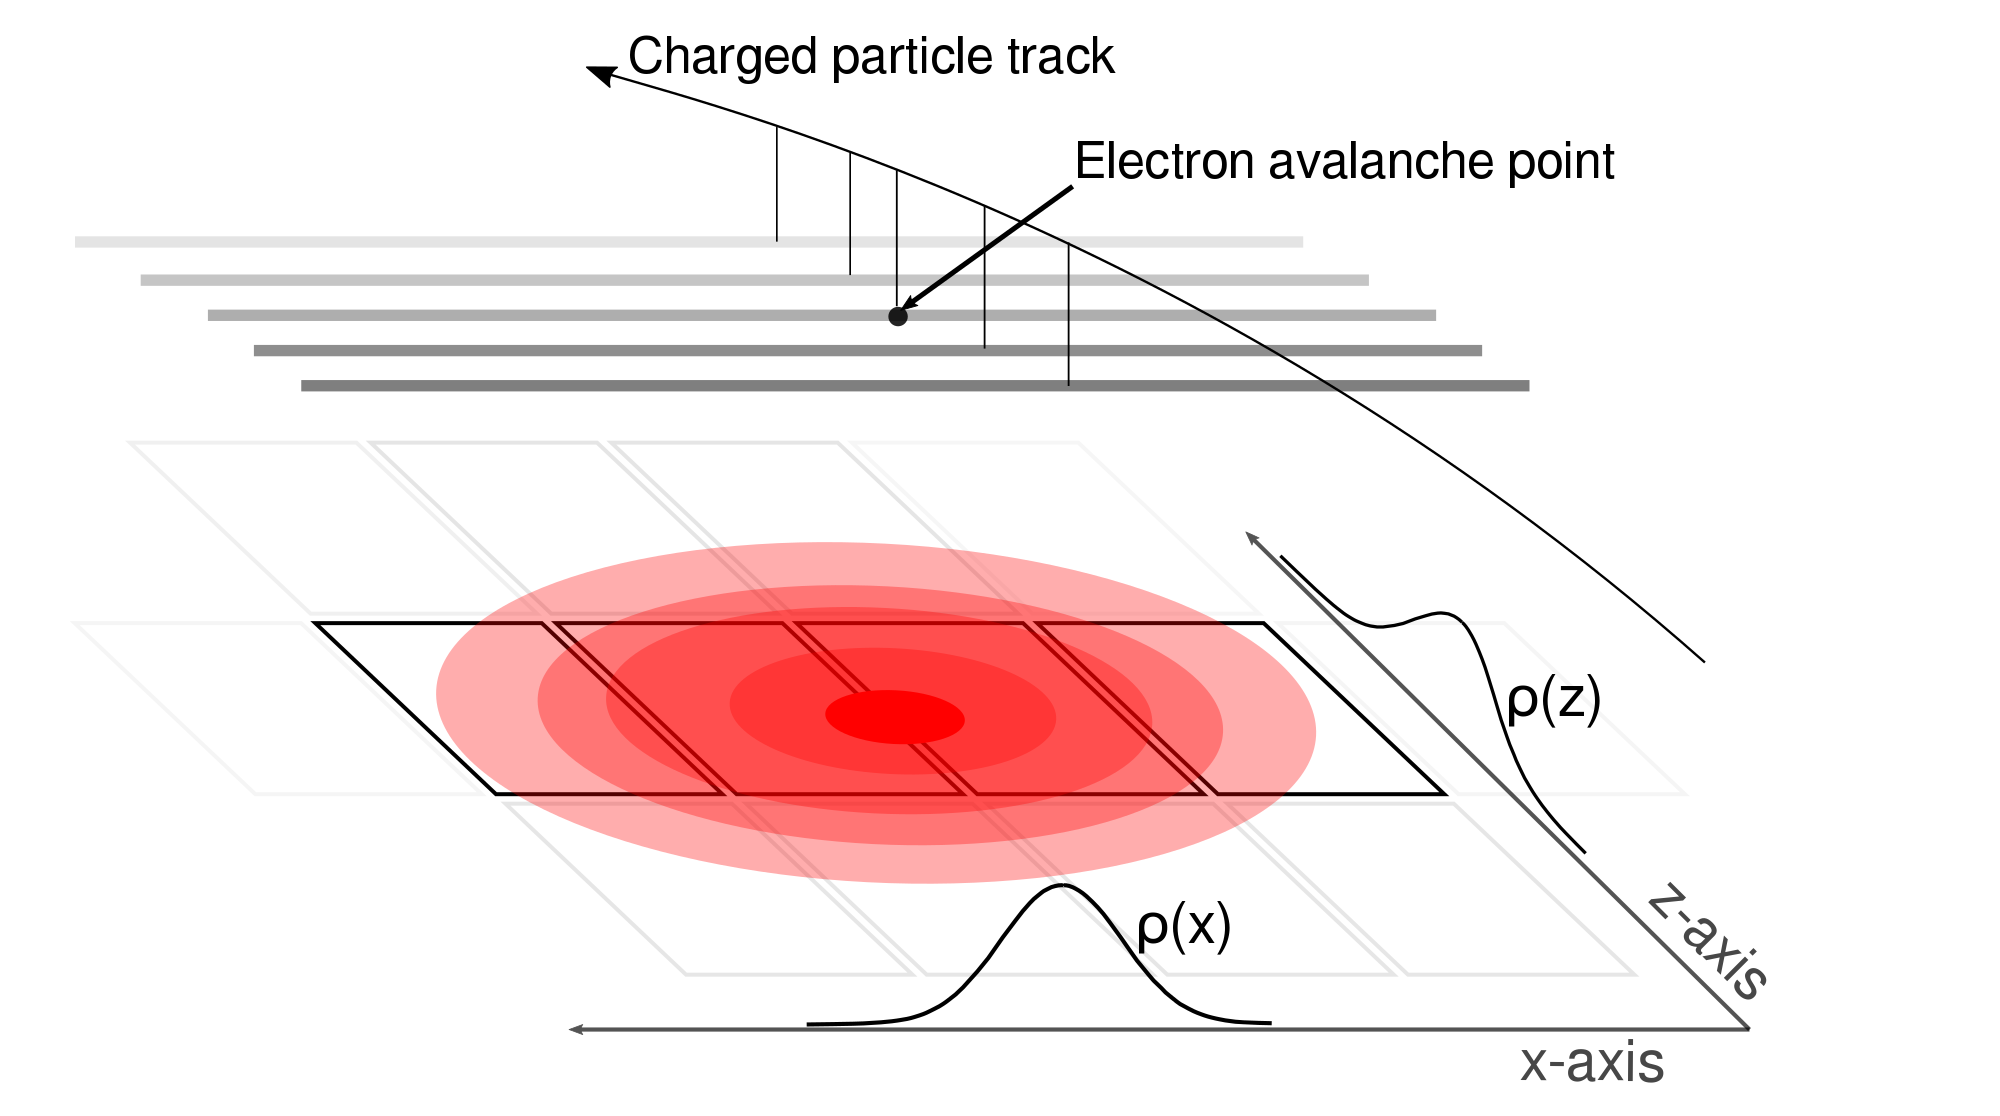
\includegraphics[width=\linewidth]{padsat_Large}
\caption{A cartoon illustration of the charge distribution resulting from an electron avalanche on one wire and the projections of the distribution onto the two axis $\rho(x)$ onto the x-axis and $\rho(z)$ onto the z-axis. The orientation of the wire planes is flipped upside down to display the perspective better.}
\label{fig:2DPRF}
\end{figure}

Gatti \cite{gatti} derived a semi-empirical formula for the charge distribution in a simple multi-wire TPC given as, 
\begin{equation}\label{eq:gatti}
\begin{split}
PRF_{\mathrm{Gatti}}(\lambda)
& = \frac{K_{1}}{K_{2}\sqrt{K_{3}}}\bigl[\arctan(\sqrt{K_{3}}\tanh\bigl[K_{2}\bigl(\frac{\lambda}{h}+\frac{w}{2h}\bigr)\bigr]) \\
& - \arctan(\sqrt{K_{3}}\tanh\bigl[K_{2}\bigl(\frac{\lambda}{h}-\frac{w}{2h}\bigr)\bigr])\bigr] \\
\end{split}
\end{equation}

where $w$ is the width of the pad, $h$ is the distance of the anode plane to the pad plane, and $\lambda$ is the distance of the pad center to the avalanche point. It is a single parameter equation where the two parameters $K_1 = \frac{K_{2}\sqrt{K_3}}{4 \arctan(\sqrt{K_3})}$ and $K_2 = \frac{\pi}{2}\left(1-\frac{\sqrt{K_{3}}}{2}\right)$ depend on the parameter $K_3$, which is a function of the ratio of the anode wire diameter to the distance of the anode wires to the pad plane. $K_3$ can be looked up in a graph in \cite{blumrol} and \cite{gatti}.



\subsection{Experimental Pad Response Function}

The correlations we introduced by only clustering along one direction do not play a significant role in the particle identification, but cause deviations from the expected Gatti distribution. Also, analytic PRFs only exist for classical multi-wire TPCs. For these reasons it is useful to experimentally measure the PRF and fit it with an empirical function, typically a Gaussian, to describe its behavior. 

As in Fig.~\ref{fig:topview}, we postulate that the PRF is a function of the total charge deposited in a cluster $Q = \sum_i q_i$, and the difference in position of the center of the $i^{th}$ pad, $x_i$, to the mean position $\bar{x} = \sum_i x_i q_i/Q$, defined as $\lambda_i = x_i-\bar{x}$. The PRF is simply defined as the charge fraction of each pad as a function of $\lambda$, as shown in Equation \ref{eq:prf}. 

\begin{equation}\label{eq:prf}
PRF(\lambda_i) = \frac{q_i(\lambda_i)}{Q}
\end{equation}

Averaging over many events in the experimental data, the resulting PRF for the S$\pi$RIT TPC is shown in Fig.~\ref{fig:expprf}. Here we see the deviations from the expected analytic Gatti distribution (black curve), whereas fitting with a two parameter Gaussian function (red curve) gives a better description of the  data, Eq.~\ref{eq:gaus}, with the two parameters being the normalization coefficient, $N_0$, width $\sigma$, and with a mean value assumed to be 0.

\begin{equation}\label{eq:gaus}
PRF_{\mathrm{Gaus}}(\lambda) = N_0 e^\frac{-\lambda^2}{2\sigma^2}
\end{equation}

\begin{figure}[ht!]s
\begin{overpic}[width=\linewidth]{fig5.pdf}
\put(61,55){\contour{white}{ PRF${}_{\mathrm{Gaus}}(\lambda)$ eq. \ref{eq:gaus}  }}
\put(61,49){\contour{white}{ PRF${}_{\mathrm{Gatti}}(\lambda)$ eq. \ref{eq:gatti} }}
\end{overpic}
\caption{Experimental pad response function of many events for a crossing angle of $85^{\circ} < \theta \leq 90^{\circ}$.  }
\label{fig:expprf}
\end{figure}

The shape of the PRF depends on the crossing angle of the track \cite{gatti}. Plotted in Fig.~\ref{fig:prfpimData} is the PRF of $\pi^-$ tracks vs. the crossing angle $\theta$. The PRF gets wider starting from $90^{\circ}$  and going to $45^{\circ}$; if we did not switch clustering directions the PRF would become wider until it was a uniform distribution and there was no position resolution. Since we switch the clustering direction from $x$ to the $z$ direction at $45^{\circ}$, the opposite trend is seen where the PRF becomes narrower as the position resolution gets better going from $45^{\circ}$ to $0^{\circ}$.




\begin{figure}[!htb]
     \centering
	 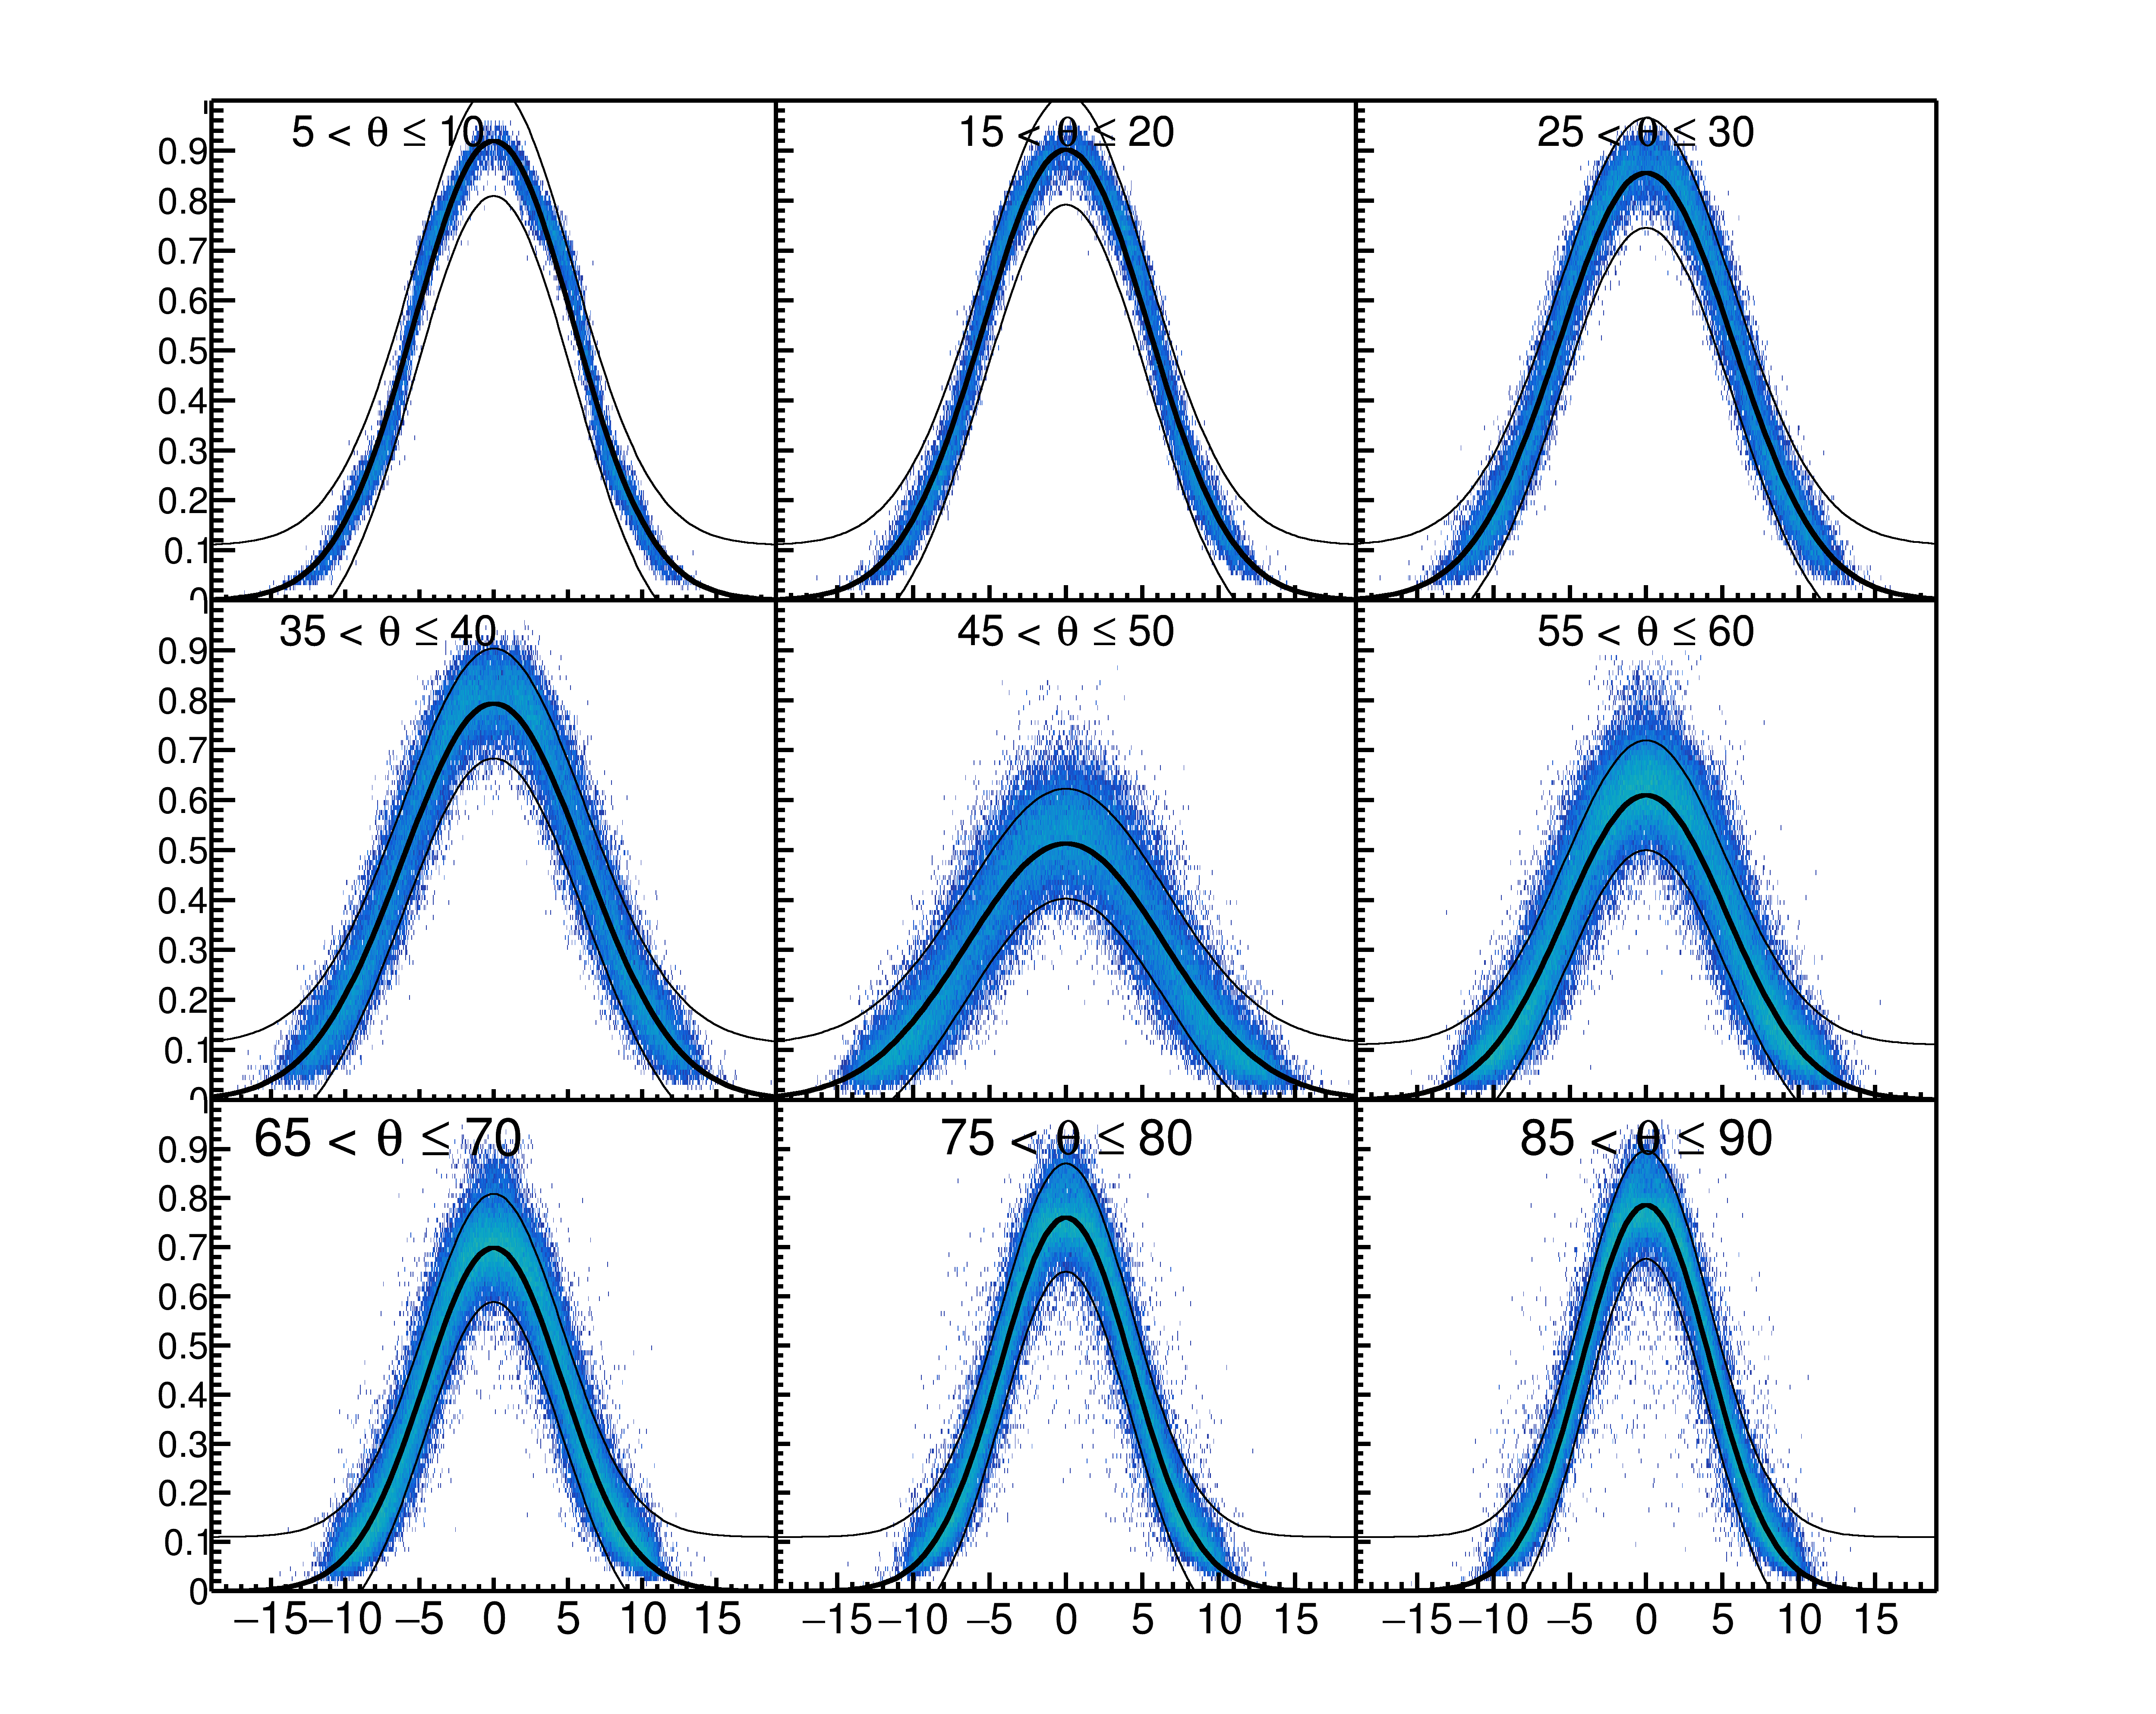
\includegraphics[width=\textwidth]{PRFs_data_wcut.png}
     \caption{PRF response from $\pi^-$ data. }
     \label{fig:prfpimData}
\end{figure}

\begin{figure}[ht!]
\vspace{5mm}
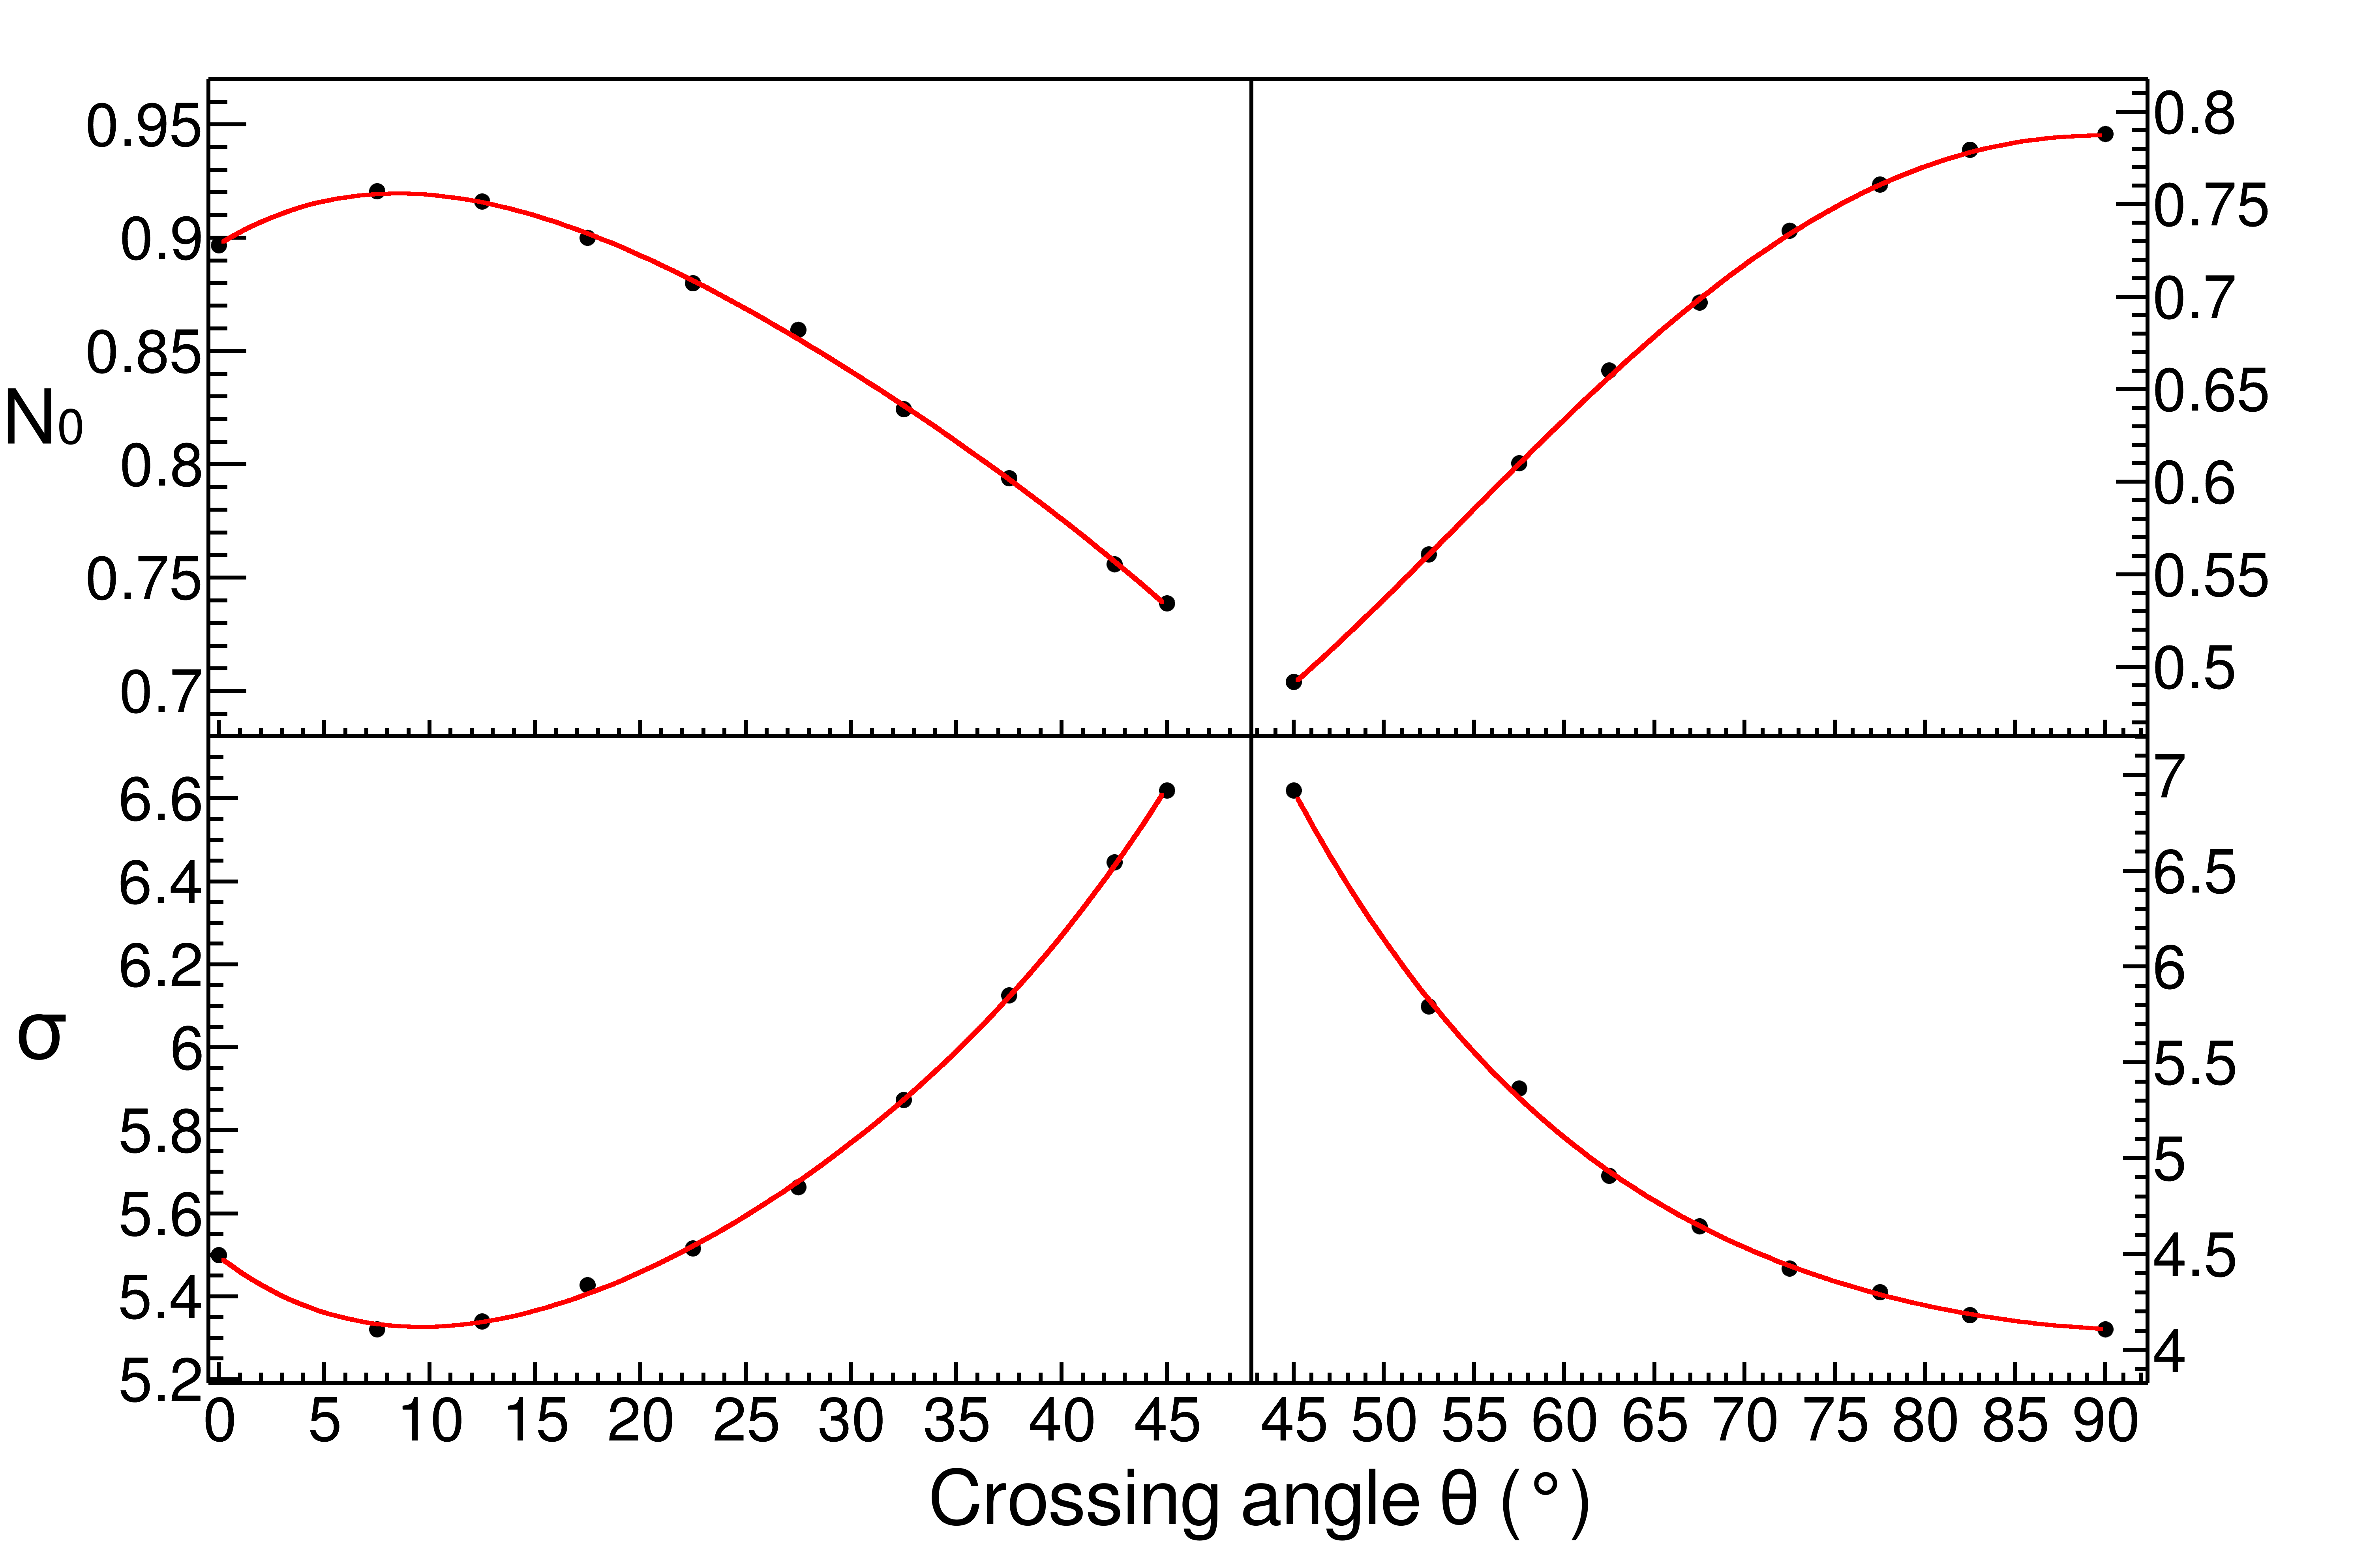
\includegraphics[width=\linewidth]{fig7}
\caption{Parameters $N_{0}$ and $\sigma$ as a function of the crossing angle $\theta$ with the $4^{th}$ order polynomial fits.}
\label{fig:normsigma}
\end{figure}

\begin{comment}
\begin{table}
\centering
 \begin{tabular}{||c c c c c c||} 
 \hline
 Coefficient & $c_0$ & $c_1$ & $c_2$ & $c_3$ & $c_4$ \\ [0.5ex] 
 \hline\hline
 $0 < \theta < 45$ & & & & &  \\ [.25ex]
 \hline
 $N_0$ & .897 & 5.766E-3 & -4.263E-4 & 7.444E-6 & 5.705E-8 \\ 
 \hline
 $\sigma$ & 5.496 & -3.920E-2 & 2.693E-3 & -5.208E-5 & 5.334E-7\\
 \hline
 $45 < \theta < 90$ & & & &  & \\ [.25ex]
 \hline	
 $N_0$ & 1.220 & -6.258E-2 & 1.608E-3 & -1.492E-5  & 4.654E-8 \\
 \hline
 $\sigma$ & 31.368 & -1.109 & 1.779E-2 & -1.336E-4 & 3.940E-7\\
 \hline
\end{tabular}
\caption{Coefficients of the $4_th$ order polynomial fit to the Gaussian parameters $N_0$ and $\sigma$. The polynomial form is given as $c_0 + c_1 x + c_2 x^2 + c_3 x^3 + c_4 x^4$}
\label{tb:coeff}
\end{table}
\end{comment}
 
Fits were performed to the experimental data with  $5^{\circ}$ width bins from $0^{\circ} < \theta \leq 90^{\circ}$. The two parameters of the Gaussian fits are plotted versus $\theta$ in Fig.~\ref{fig:normsigma}; a $4^{th}$ order polynomial fit between these points allowed for interpolating between $\theta$.




\section{S$\pi$RIT TPC Overview}
%Add Overview image with labels
The Samurai Pion-Reconstruction and Ion Tracker Time Projection Chamber (S$\pi$RI TPC) is a Multi-Wire Proportional Counter developed to measure pions and other light charge particles resulting from radioactive heavy ion collisions in a fixed target experiments.  The TPC is enclosed in a thin aluminum sheet walls all around in order to minimize neutron scattering and to allow for light charged particles to reach the arrays of scintillating bars detectors on the sides and downstream of the TPC. The S$\pi$RI TPC was developed to fit inside the Samurai dipole magnet used at the Rare Isotope Beam Factory (RIBF) at RIKEN in Wako-shi, Japan \cite{riken}; the dipole gap limited the vertical space of the TPC. More detail and specifications of the Samurai dipole magnet are given in \cite{samurai}. 

A target ladder allowed for up to 5 fixed targets to be mounted. A ACME worm gear allowed for the x-axis motion for changing the targets during the experiment, without needing to open or move the TPC. The motion of this worm gear was translated through the target motion feed-through by several brass gears and non-magnetic gear boxes. The motion of the target ladder could be controlled by hand or by operation of the drill. The targets were mounted on stand-offs on the target ladder and also had z-axis motion. This allowed for the targets to be positioned as close as possible to the thin window of the field cage, maximizing the geometric acceptance. 

The electronics were mounted to the aluminum top plate. Several aluminum ribs were mounted to the top of the plate to bring structural rigidity. A flatness within 150$\mu$m was achieved across the whole top plate as measured by a laser position system. The charge sensitive pads of the pad plane were etched into several circuit boards were recessed and glued to the bottom portion of the top plate. Vias through the pad plane circuit boards brought the signal traces from the pads to surface mount pads on the other side of the boards. Several holes cut through the top plate allowed for the interface cables of the electronics to be connected to these surface pads. 

Just below the pad plane were a set of three wire planes; the gating grid, ground, and anode wire planes. The detailed function of these wires will be explained later but they served to separate the boundary between the drift volume and the avalanche volume. 

The front and sides of the field cage were assembled from 8 independent rigid circuit boards. The downstream window served as the downstream wall of the field cage all though it was was a large polycarbonate frame in which a removable kapton window could be installed. This thin window minimized the scattering of exiting neutrons and charged particles for downstream detectors. 

The voltage step down takes the high voltage of the field cage cathode and steps the voltage down through a set of copper rings and a resistor chain, minimizing the chance for sparking. 

\begin{table*}\centering
\ra{1.3}
\begin{tabular}{@{}rr@{}}\toprule 
\multicolumn{2}{c}{\spirit TPC Overview} \\
 \midrule
Pad plane area & 1.3 m x .9 m\\
Pad size       & 1.2 cm x .8 cm \\
Number of pads & 12096 (112 x 108) \\
Gas composition& 90\% Ar + 10\% CH${}_4$  \\
Multiplicity limit & 200  \\
dE/dx range        & Z=1-8, $\pi$, p,d,t,He,Li-O \\
Drift length       & 50 cm \\
\bottomrule
\end{tabular}
\caption{An overview of the properties of the \spirit TPC}
\label{tb:spiritoverview}
\end{table*}



\begin{figure}[!htb]
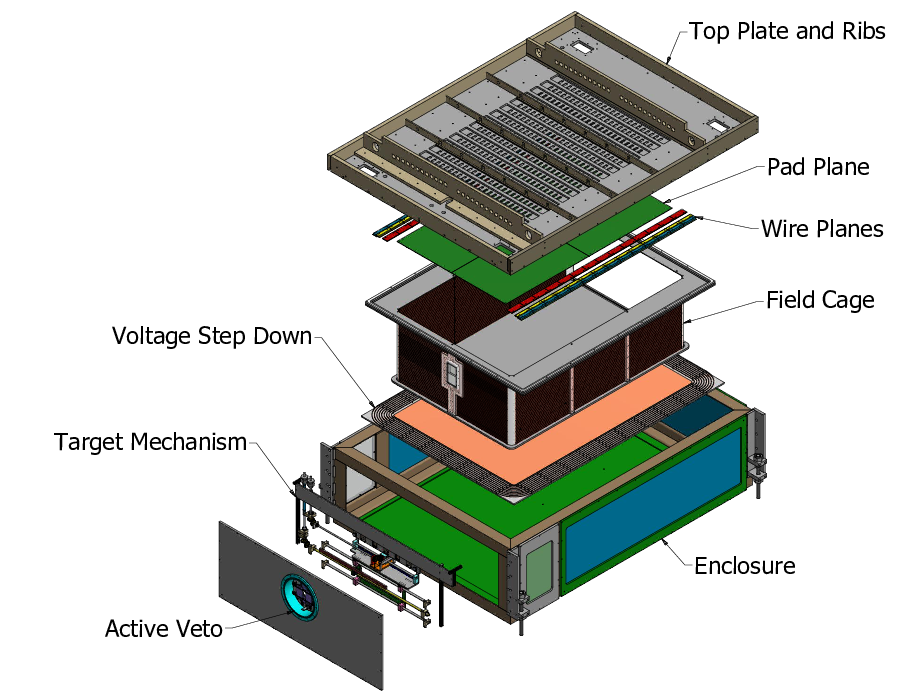
\includegraphics[width=\textwidth]{exploded.png}
\caption{Overview of the \spirit TPC}
\label{fig:tpcExplode}
\end{figure}

\subsection{Enclosure}
The skeleton of the enclosure is composed of a rigid aluminum angle-iron frame. All walls are constructed of a aluminum frame with think sheet metal. All materials were made to be as thin to allow charged particles and neutrons to exit the TPC without scattering too much. This allows for a trigger to be created by placing detectors on the sides and downstream of the TPC. The enclosure itself is made to be gas tight with respects to the outside and the field cage. This is to allow for the possibility to run a different gas inside the enclosure than the field cage. Although, in this set of experiments we ran the same gas in the field cage and enclosure volume. 

\subsection{Voltage Step Down}
The gap between the field cage's cathode and the ground of the enclosure is quite small. To prevent electric breakdown in the gas between this gap a series of concentric copper rings safely stepped down the voltage to ground; where each ring was separated by a resistor. There were 7 concentric rings with a \SI{10}{\mega\ohm} resistors in between, creating a resistor chain which steps down the voltage each ring by approximately \SI{1000}{\volt}.

\subsection{Field Cage}

The field cage holds the detector gas and sets up a uniform electric field in which electrons can drift upwards toward the anode wires. It was designed to hang from the top plate and therefore needed to be of a lightweight construction. Also the materials needed to be thin to allow for light charged particle and neutrons to pass through without significant scattering for ancillary detectors. Therefore instead of a downstream wall, a large thin exit window was constructed. The cathode was constructed of an aluminum honeycomb laminate. Two sheets of ??? aluminum were bonded to a core of aluminum honeycomb structure providing a lightweight yet rigid structure for the cathode. 

\begin{figure}[!htb]
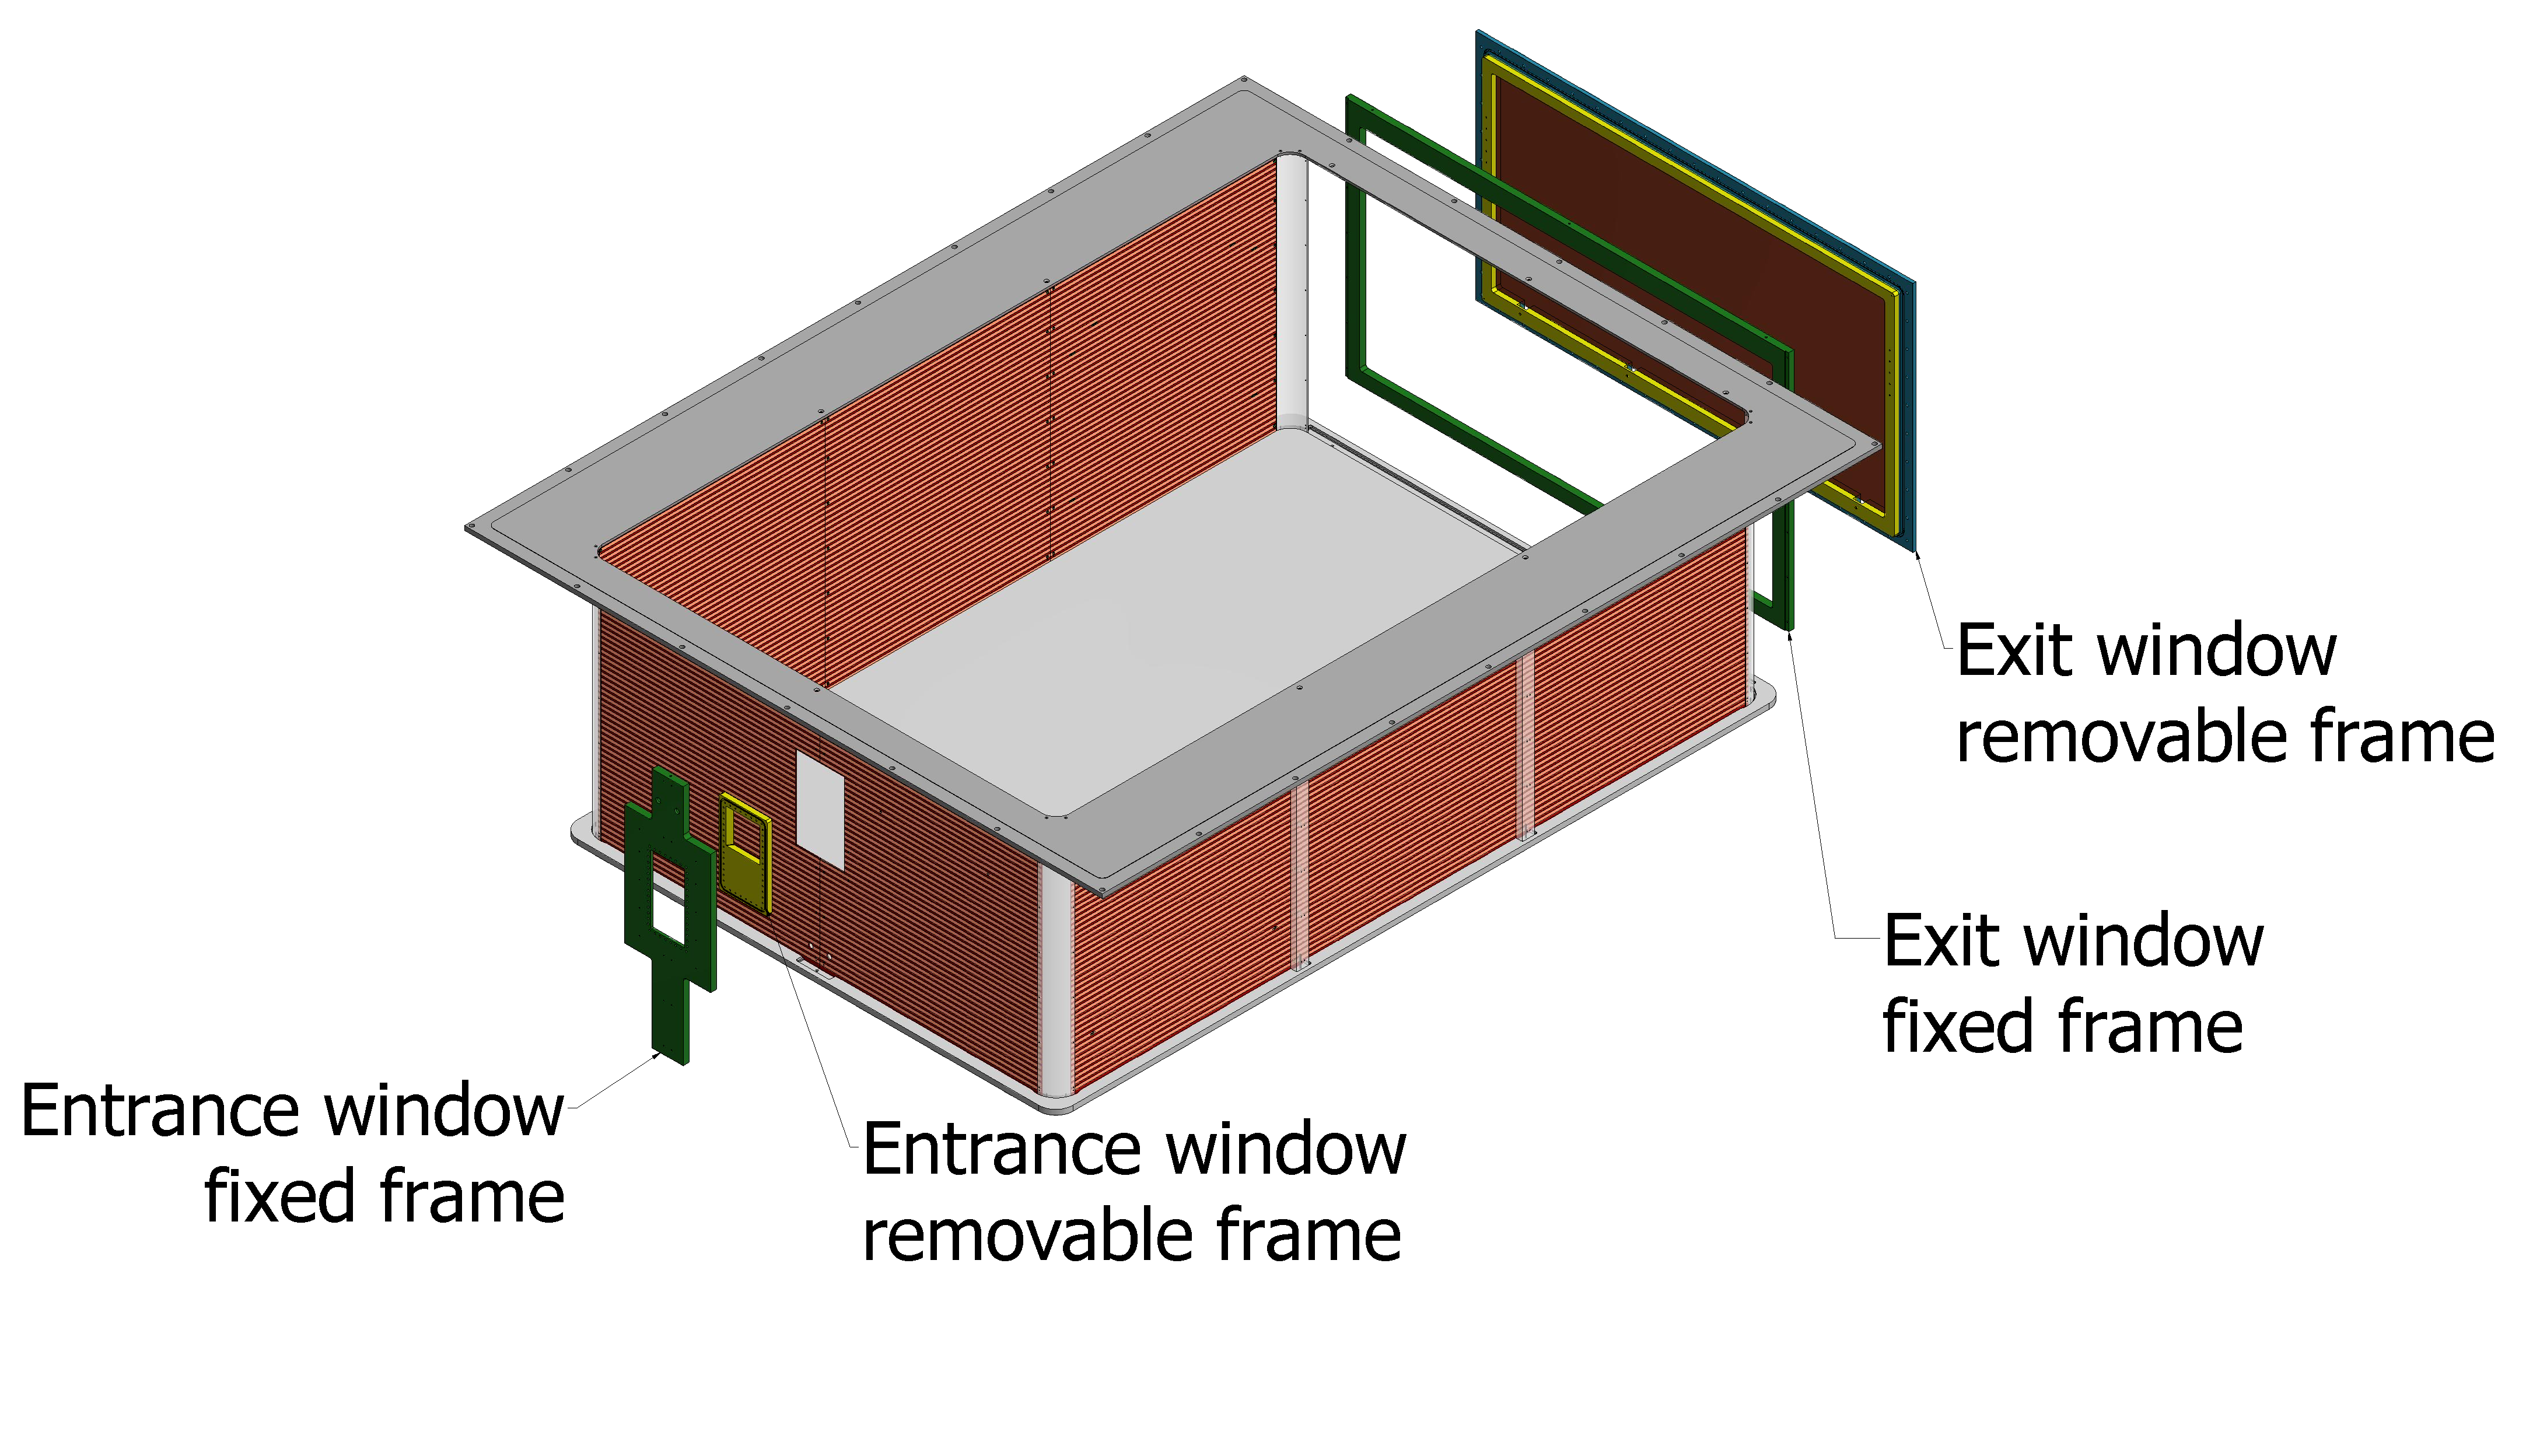
\includegraphics[width=\textwidth]{fc_overview.pdf}
\label{fig:fc_overview}
\caption{FC overview}
\end{figure}


\begin{figure}[!htb]
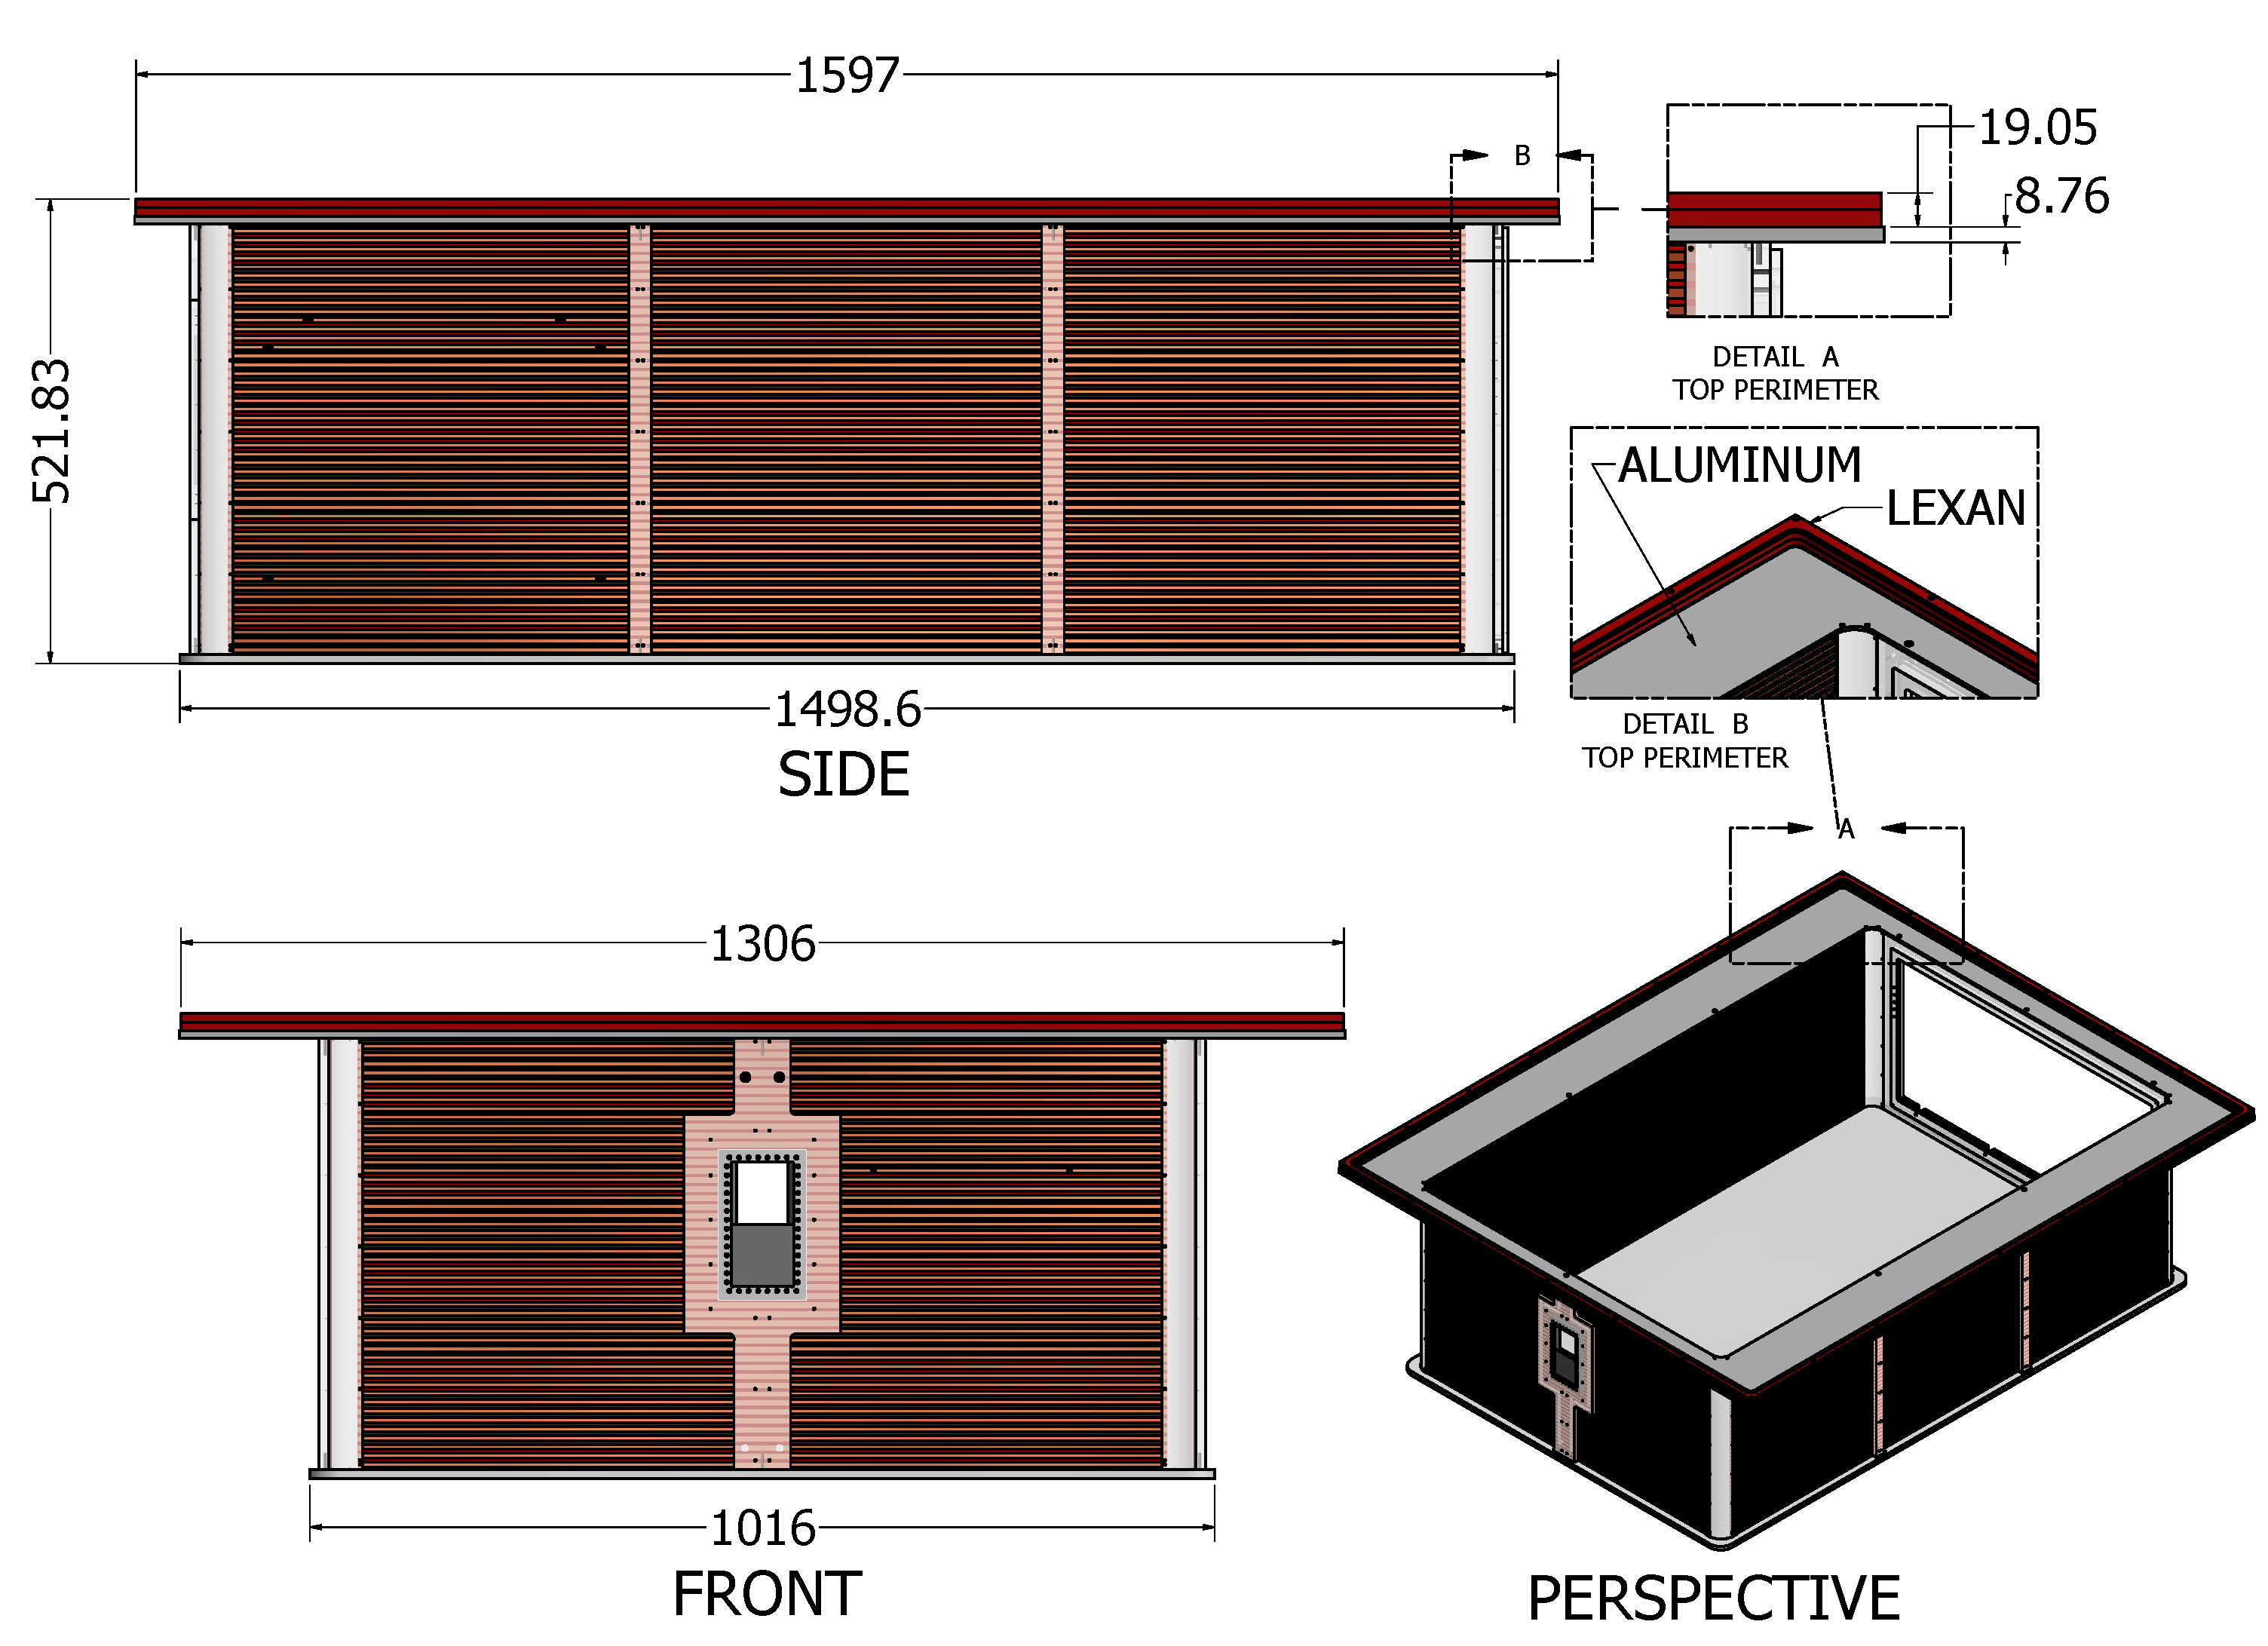
\includegraphics[width=\textwidth]{fc_overview2.pdf}
\label{fig:fc_overview2}
\caption{FC overview 2}
\end{figure}

The field cage was constructed from several panels of printed circuit boards (PCBs). The epoxy in the common PCB substrate FR4 contains bromine which is not suitable for the long term operation of a TPC, as the bromine will eventually cause gain reduction of the wires [CITE]. The halogen free material chosen was Cryogenic-G10. We built the TPC with the option to run explosive gases such hydrogen, thus we decided to have field cage an isolated volume from the rest of the TPC enclosure. While the risk of a high voltage spark was minimized using the voltage step down, the risk of sparking when using an explosive gas could be further minimized by isolating the detector volume from the enclosure volume thereby allowing you to run an insulating gas between the field cage while running the explosive gas inside the detector volume only.  

The front of the field cage was made of two PCBs and each side was constructed of three PCBs. The exit window was a 10$\mu$m thick Kapton window with evaporated aluminum strips on the inside and outside; mounted on a polycarbonate frame.


\begin{equation}
V_n = V_{cath} \frac{R_p + (50 - n)R}{49\cdot R + R_p}
\label{eq:FCstrip}
\end{equation}

\begin{equation}
R_p = 49 \cdot R  \left(\frac{ y_{g.g.} - y_{cath} }{ y_{TP} - y_{cath} \frac{V_{cath} - V_{gg}}{V_{cath}} }- 1 \right)
\label{eq:TP_resistor}
\end{equation}

\begin{figure}[!htb]
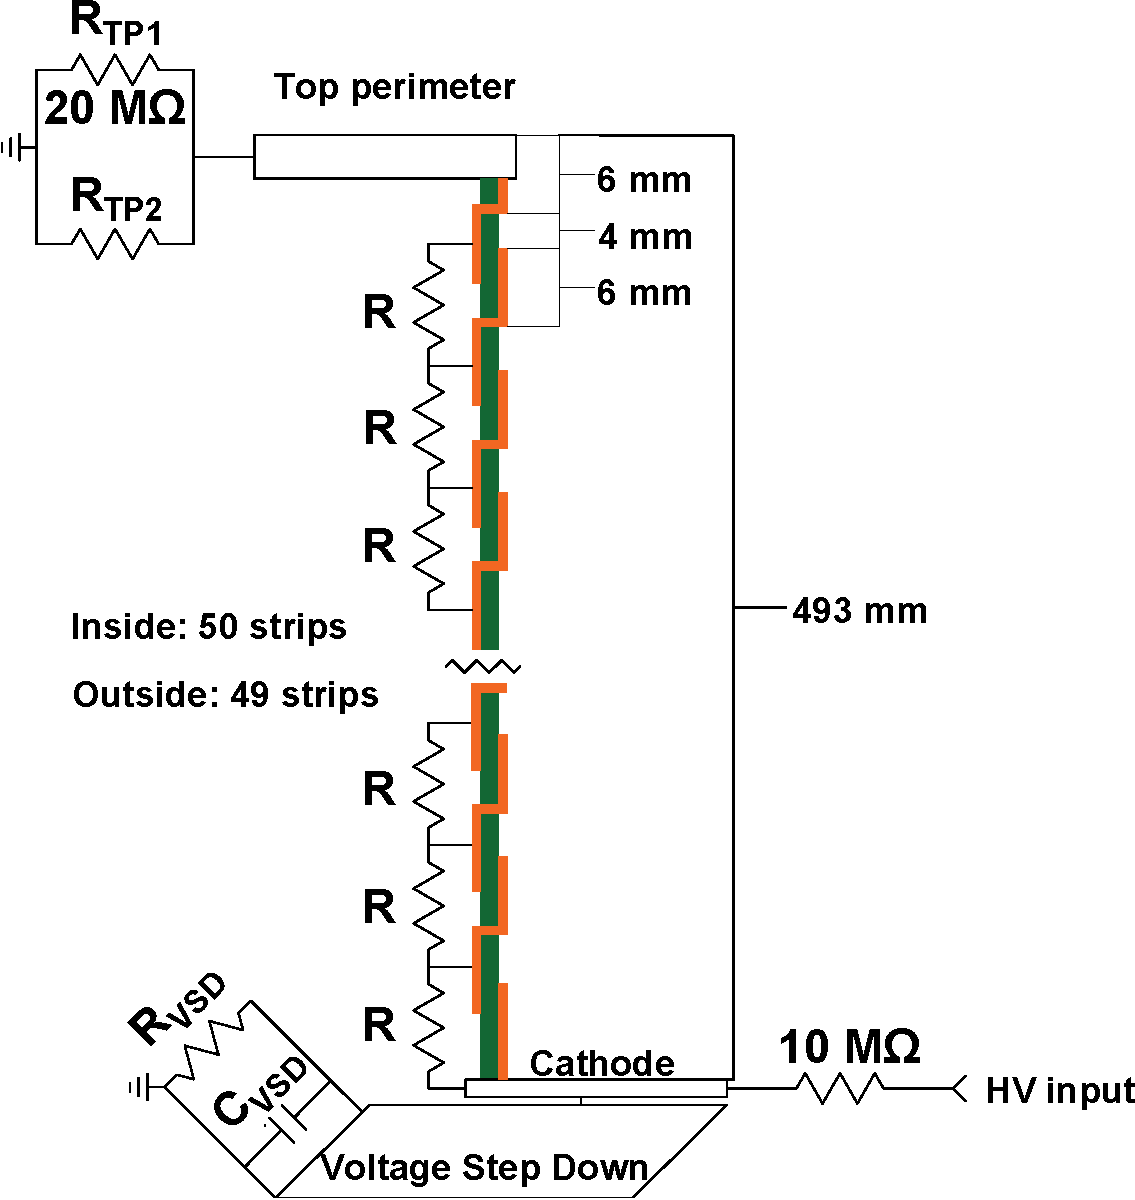
\includegraphics[width=\textwidth]{FC_schematic.pdf}
\label{fig:FC_schematic}
\caption{Schematic of the electric connections relevant to the Field Cage system.}
\end{figure}
\subsection{Voltage Step Down}



\begin{figure}[!htb]
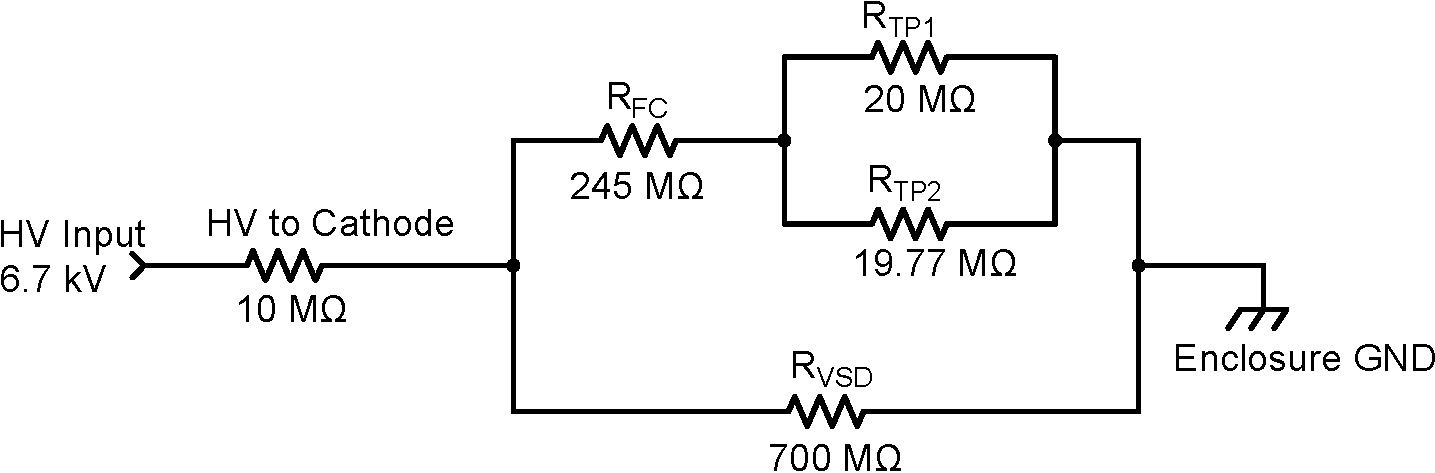
\includegraphics[width=\textwidth]{TPC_schematic.pdf}
\caption{Schematic of the TPC system}
\label{fig:TPC_schematic}
\end{figure}

Figure~\ref{fig:FC_schematic} shows a cartoon drawing of the electrode geometry of the field cage walls. The basic idea of the field cage is to set up a constant electric field in the field cage volume to allow for a constant drift, in the presence of gas, for electrons. To accomplish this the field cage is composed of a set of copper strips which are set at a defined voltage by a resistor chain for a fixed distance between strips; setting up a constant electric field. 

The cathode itself is connected to the HV supply through a \SI{10}{\mega\ohm} resistor and has an effective capacitance to ground of \SI{4}{\nano\farad}, $C_{VSD}$. The field cage is made of 50 inside copper strips and 49 outside copper strips; the strip thickness is exaggerated in the figure to show the detail. The first inside strip is connected to the cathode which is connected by an effective \SI{5}{\mega\ohm} resistor, $R$, to the next inside strip and the first outside strip. The resistor chain creates a voltage divider in which each strip is separated by a constant difference voltage at a fixed distance setting up a constant electric field. The last strip of the field cage is composed of partially a small inner strip on the PCB board and the aluminum top perimeter piece which holds the field cage together with the top plate of the TPC. Together their thickness is equal to the \SI{6}{\milli\metre} strip width of the other strips. The top perimeter is connected to electrical ground through a \SI{20}{\mega\ohm} resistor with the option to place an additional resistor in parallel to tune the voltage of the top perimeter. 



\subsection{Pad Plane}
Add figure of close up of pad plane 


\subsection{Wire Planes}
%Add figure of gating grid transparency closed and open configuration 
There are three wire planes that sit underneath the pad-plane. The wire plane closest to the pad-plane (\SI{4}{\milli\metre}), is the anode wire. The next plane (\SI{12}{\milli\metre}), is the ground plane or frisch grid, and the last plane (\SI{14}{\milli\metre}), is the gating grid. The gating grid is the first plane that electrons meet as they drift upward towards the anode plane. The gating grid is operated as a gate either allowing electrons and ions through or blocking them entirely. The ground plane shields the inside volume of the TPC from the high voltages of the anode wires where the avalanche process of the electron takes place. 

The ground plane is the least interesting plane and is shorted to the enclosure ground by a BNC terminator on the outside of the TPC. If we would like to calibrate the electronics of the TPC we typically inject a pulser into one end of the ground plane and terminate the other end with a \SI{50}{\ohm} termination. 

In the open configuration the gating grid is transparent to electrons coming from the TPC volume and also allows for ions to move from the avalanche region into the TPC volume. It functions as the gate of the TPC where we only open the gating grid when an event meets the selection trigger criteria; minimizing the excessive exposure to the un-reacted beams which would quickly build up enormous amounts of space charge. We close the TPC after reading out approximately one TPC volume -- about \SI{10}{\micro\second}  -- of space to prevent the back-flow of ions from the avalanche region of that event. Since ions move with a velocity much slower than that of elections, the ions only move several \si{\micro\metre} in the time the gate is open; this allows for electrons to pass through while preventing the back-flow of ions into the FC volume. Figure~\ref{fig:gg_onoff} shows a Garfield simulation of the gating grid in both the on and off configurations. In the on configuration, all the wires share the same average voltage, $V_{g.g.}$, which is optimized for the case of 100\% electron transparency. In the off configuration the reference voltage $V_{g.g.}$ remains the same, but alternating wires get an offset voltage of $\pm \Delta V$, so that the electric field between wires is great enough to block incoming electrons; opening the grid from this closed bi-polar mode is simply done by removing the offset voltage and allowing the two wires to connect and equilibrate their charges back to the reference voltage. 


\begin{figure}
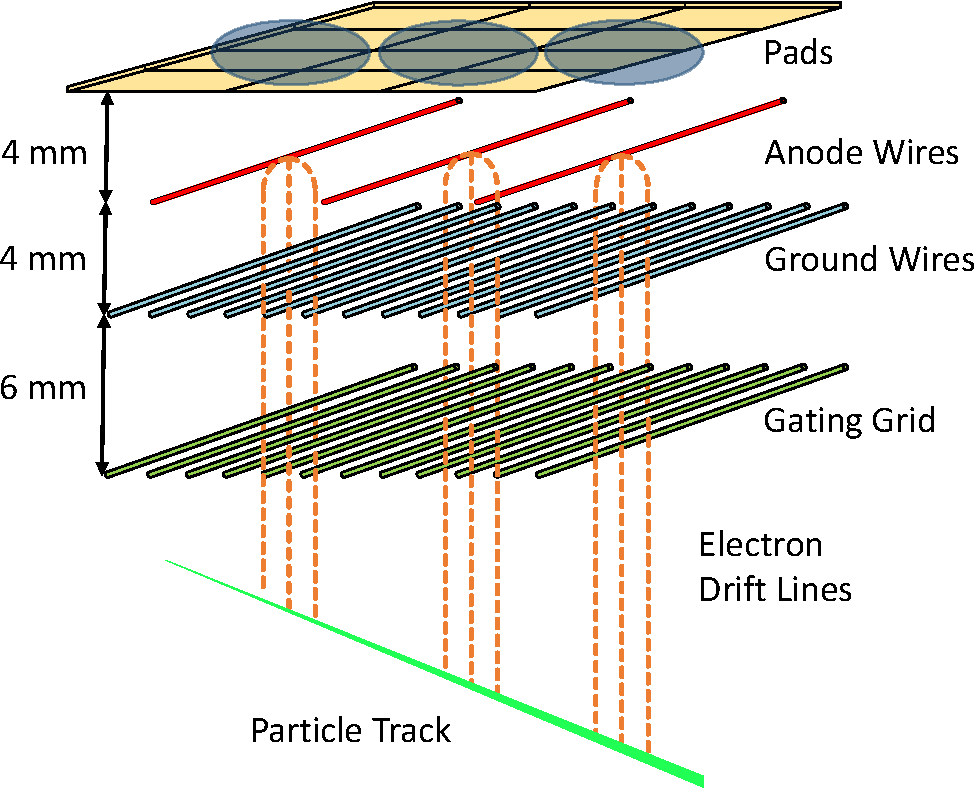
\includegraphics[width=\textwidth]{wires_open.pdf}
\caption{Cartoon graphic of the wire plane structures}
\label{fig:wires_open}
\end{figure}


\begin{figure}[!htb]
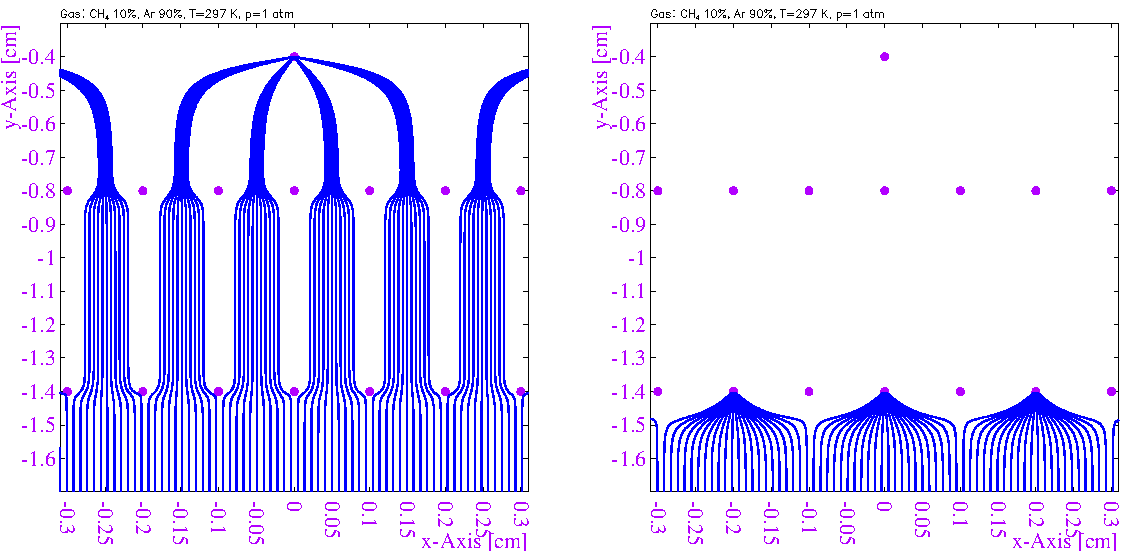
\includegraphics[width=\textwidth]{gg_onoff.pdf}
\caption{On and off configurations of the gating grid.}
\label{fig:gg_onoff}
\end{figure}

The anode wires are typically biased to \SI{e3}{\volt} and are very thin, about \SI{20}{\micro\metre} in diameter. This creates a very high electric field very close to the anode wire in which the electron gains significant kinetic energy producing electrons until it terminates on the anode wire. The amount of electrons it produces depends on the anode wire voltage and the gas properties. The absolute gas gain was not experimentally measured but was simulated by a Garfield simulation. During the experiment the anode wires were biased to two different voltages. We will refer to the voltage \SI{1460}{\volt} as the ``high voltage" and \SI{1214}{\volt} as the ``low voltage". Only two sections were biased with the lower voltage setting due to concerns of a high current issue. Figure~\ref{fig:anodegain} shows the expected number of electrons distributions for electrons produced in a avalanche process of an electron creating a single avalanche. The distribution follows a Polya distribution as expected and the MC data in the simulation was fit with a Polya function \cite{blumrol}. 

 
\begin{figure}[!htb]
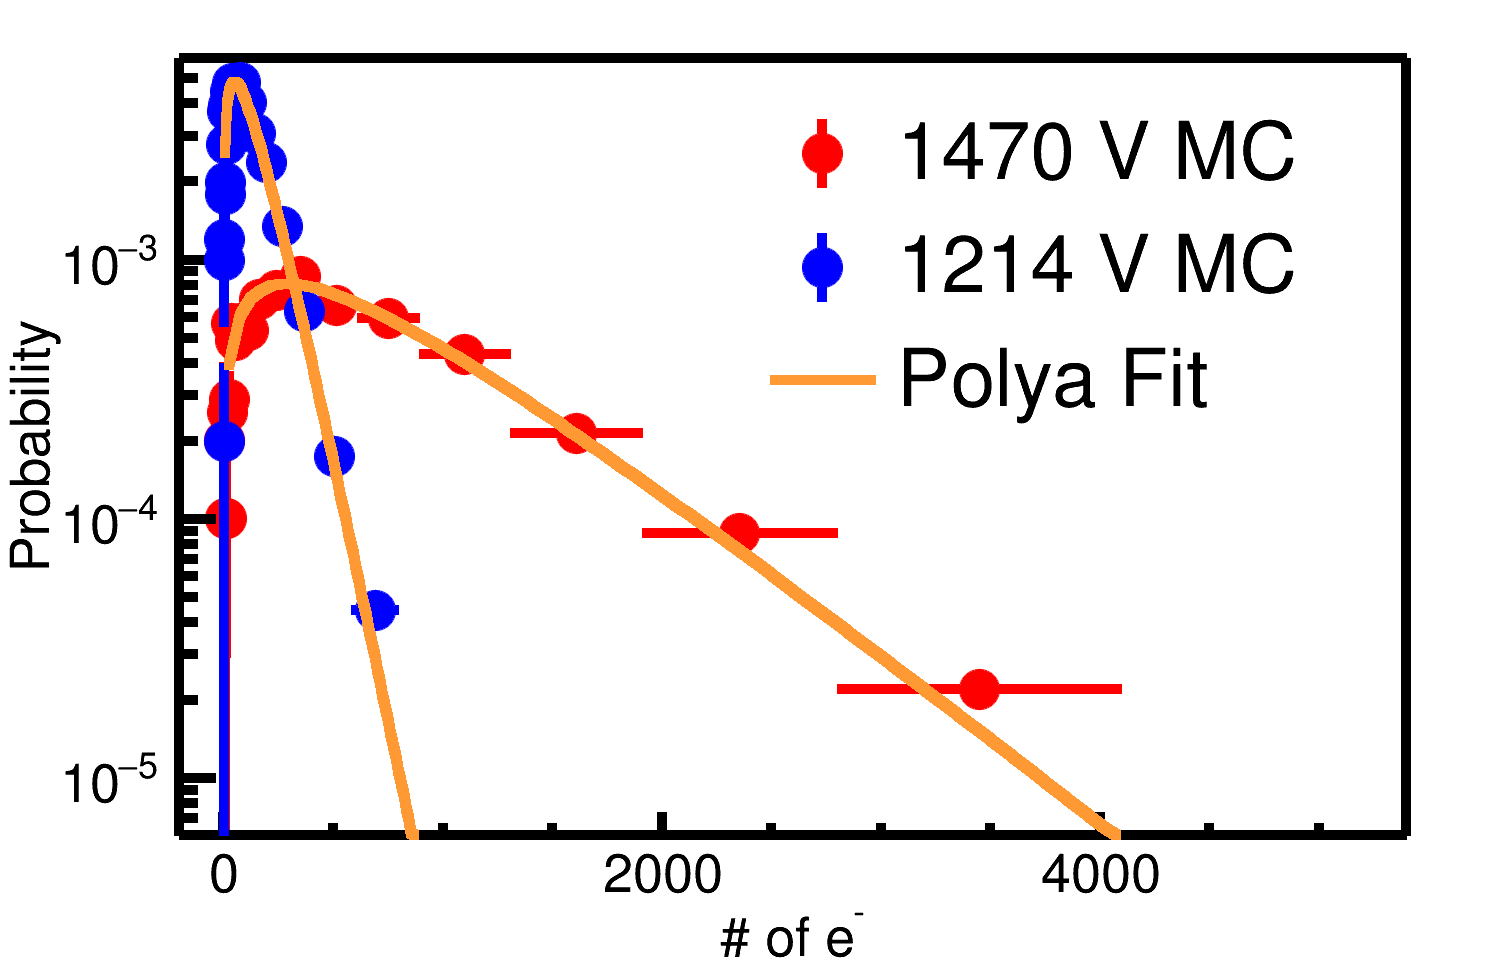
\includegraphics[width=\linewidth]{gain.png}
\caption{Number of electrons produced in a single avalanche on an anode wire. Two different voltages were simulated using Garfield++ at 1470 $V$ and 1214 $V$. The expected Polya distribution fit is also given in yellow.}
\label{fig:anodegain}
\end{figure}


\subsection{Electronics}

Signals in the S$\pi$RIT TPC are amplified and digitized by the recently developed Generic Electronics for TPCs (GET) \cite{get}.  Short cables transmit the signals from the pads to the inputs of the AGET chips. Each AGET chip services 64 pads (63 pads are connected in our case), contains a pre-amplifier, and a Switched Capacitor Array (SCA), with a maximum of 512 time buckets with an adjustable sampling frequency of 1 to 100 MHz. Four AGET chips are mounted on one AsAd (ASIC and ADC) motherboard. The gain of each AGET can be configured as 0.12, 0.24, 1.0, or 10 pC over the whole dynamic range, and the ADCs on each AsAd board provides 12 bit resolution. The peaking times of the shaping amplifiers can be set to 69, 117, 232, 501, 720, or 1014 ns. In this experiment, the gain was set to the highest setting, 0.12 pC, the peaking time 117 ns, and the sampling frequency 25 MHz (resulting in 40 ns time buckets). The Aget 2.0, asad 2.1, and cobo 1.0 firmware versions were used. The variations in the electronics were calibrated by measuring the response of each channel to a injected reference pulse, covering the full dynamic range of each channel. 


\begin{table*}\centering
\ra{1.3}
\begin{tabular}{@{}rr@{}}\toprule 
\multicolumn{2}{c}{GET electronics settings}\\
\midrule
ADC bit range       & 14 bits \\
Sampling frequency  & 1-100 MHz \\
Dynamic range       & .12, .24, 1.0, 10pC \\
Peaking time        & 69,117,232,501,720,1014 ns \\
Time bucket range   & 512\\
\bottomrule
\end{tabular}
\caption{Summary of range of GET electronics settings. }
\label{tb:getoverview}
\end{table*}

\subsection{Considerations when constructing a TPC}
Several considerations went into the construction of the S$\pi$RI TPC which I wish to summarize and document here. All materials and glues of the TPC were selected as low out-gassing materials. Several materials (that are common place in nuclear labs), such as vacuum grease, viton o-rings, all out-gas organic chemicals into the counter gas which damage the TPC by permanently lowering the gain over time. The organic molecules responsible are difficult to identify exactly, but lists of good and bad materials are well known in the literature from experiments. If a material we wished to used was not on these lists we placed the material in a clean chamber with the counter gas and flowed this counter gas through a small proportional counter making sure the gain did not drop at high collection rates when exposed to a high rate alpha Americium source. 

Sparking
Two volumes of gas. 


\subsection{Gas Properties}
The gas used inside of the field cage was a mixture of 90\% Ar and 10\% Methane ($\mathrm{CH_4}$) by volume --so called P10--  gas, operated just under atmospheric pressure (1 atm). The  gas was continually flowed through the field cage and exited into the enclosure volume, finally passing through a bubbler to atmosphere. The gas purity was monitored with an oxygen and water monitor which are the two most concerning contaminants. The water never exceed  ??? ppm  and the oxygen level never exceeded ??? ppm. Figure~\ref{fig:driftvel} shows the drift velocity of P10 gas at 1 atm as a function of electric field value in \si{\volt\per\centi\metre}. Operating near the peak value of the drift velocity curve minimizes the change in the drift velocity as the effective field slightly changes due to slight variations in the pressure. The electric field in the experiment was \SI{125}{\volt\per\centi\per\metre} at \SI{760}{\torr}, giving a reduced electric field \SI{0.17}{\volt\per\centi\metre\per\torr}.

\begin{figure}[H]
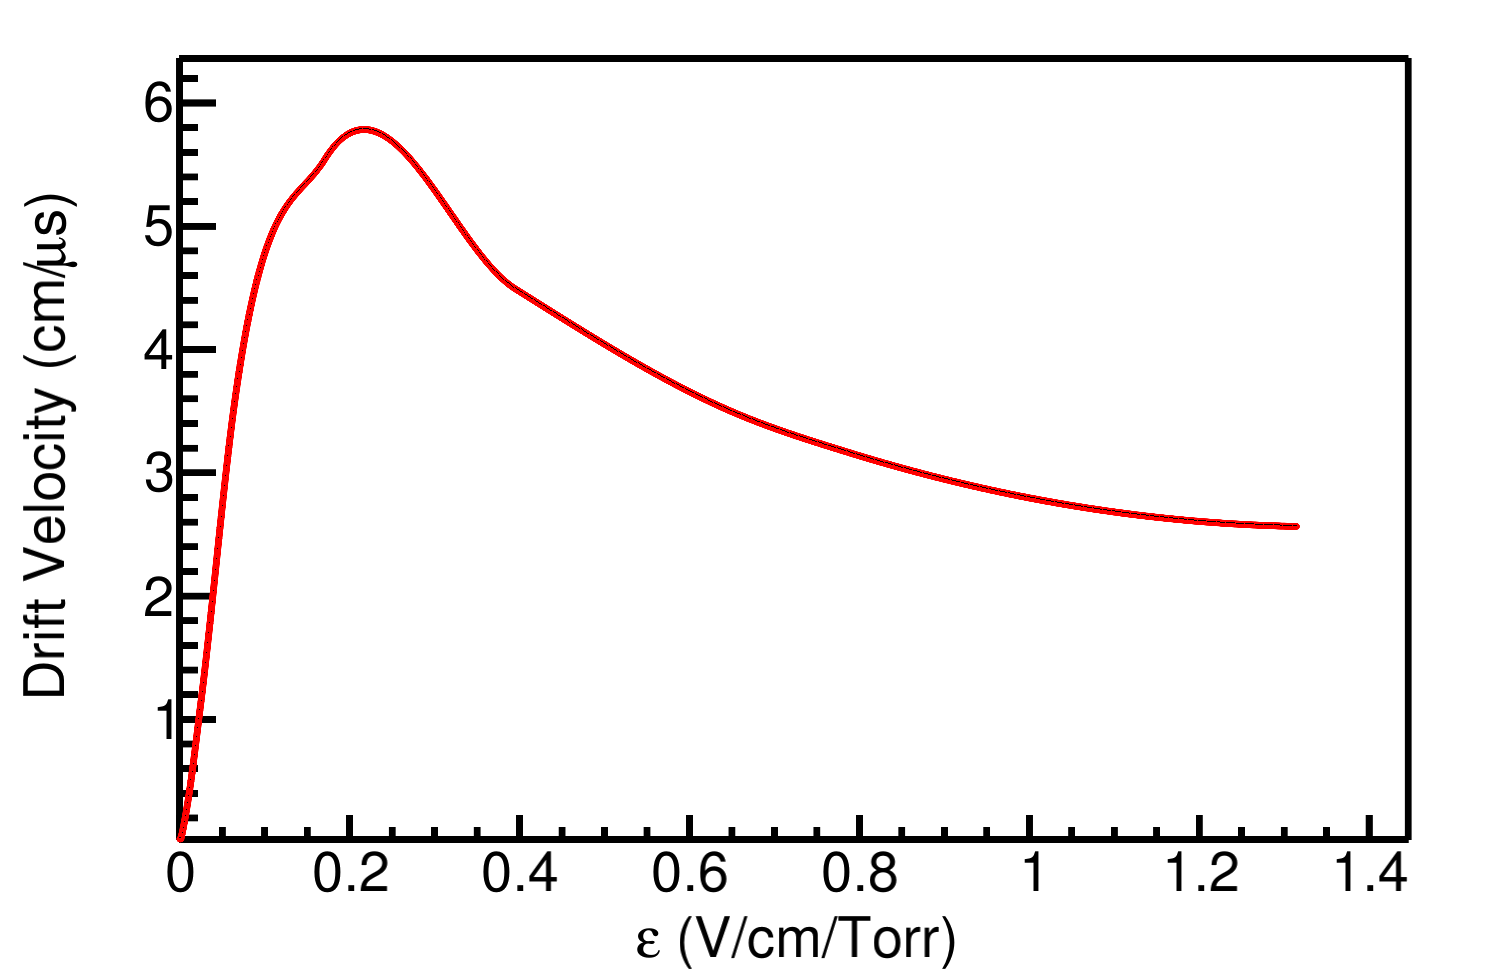
\includegraphics[width=\linewidth]{driftvel.png}
\caption{Drift velocity of electrons in P10 gas.}
\label{fig:driftvel}
\end{figure}

The general formula for the drift velocity, $d\vec{x}/dt$, of an electron in the presence of electric and magnetic fields, $\vec{E}$ and $\vec{B}$, can be expressed in the Langevin equation as,  

\begin{equation}
\frac{d\vec{x}}{dt} = \frac{\mu}{1+(\omega\tau)^2}\Big(\vec{E} + \omega\tau\frac{\vec{E}\times\vec{B}}{|\vec{B}|}+\omega^2\tau^2\frac{\vec{E}\cdot\vec{B}}{|\vec{B}|^2}\vec{B}\Big),
\label{eq:elecdrift}
\end{equation}

where $\mu$ is the signed drift velocity, $\omega$ is the cyclotron frequency, and $\tau$ is the collision parameter for a particular gas \cite{blumrol}.

Several properties of the gas were also simulated in Garfield such as the longitudinal and transverse diffusion, $sigma_l$ and $sigma_t$ respectively, and the electron and ion drift velocities, $v_d$ and $v_i$ respectively for the experimental electric field of \SI{125}{\volt\per\centi\metre}; summarized in Table~\ref{tb:gasprop}.


\begin{table}[!htp] % not just 'h!'
\centering % not a center environment
\begin{tabular}{
  @{}
  l
  S[table-format=1.2]
  S[table-format=1.2]
  S[table-format=1.2]
  S[table-format=1.2]
  S[table-format=5.2]
  S[table-format=5.2]
  @{}
}
\toprule
Gas properties &
 {$\sigma_{t}$} &
 {$\sigma_{l}$} &
 {$v_{d}$} &
 {$v_{i}$}  &
 {$G_{h}$} &
 {$G_{l}$} \\
&
  {($\si{\centi\meter}^{-1/2}$)} &
  {($\si{\centi\meter}^{-1/2}$)} &
  {(\si{\centi\meter\per\micro\second})} &
 {(\si{\centi\meter\per\micro\second})} \\

\midrule
\phantom{abc}   &.024   &.034  &5.43  &  \num{2.05e-4} &  903   &150     \\
\bottomrule
\end{tabular}

\caption{}
\label{tb:gasprop}
\end{table}


%Add table for gas diffusion 


\section{Ancillary Detectors }


\subsection{Kyoto Multiplicity Trigger}
%kyoto array sets multiplicity trigger
%scintillator bars


\begin{figure}[!htb]
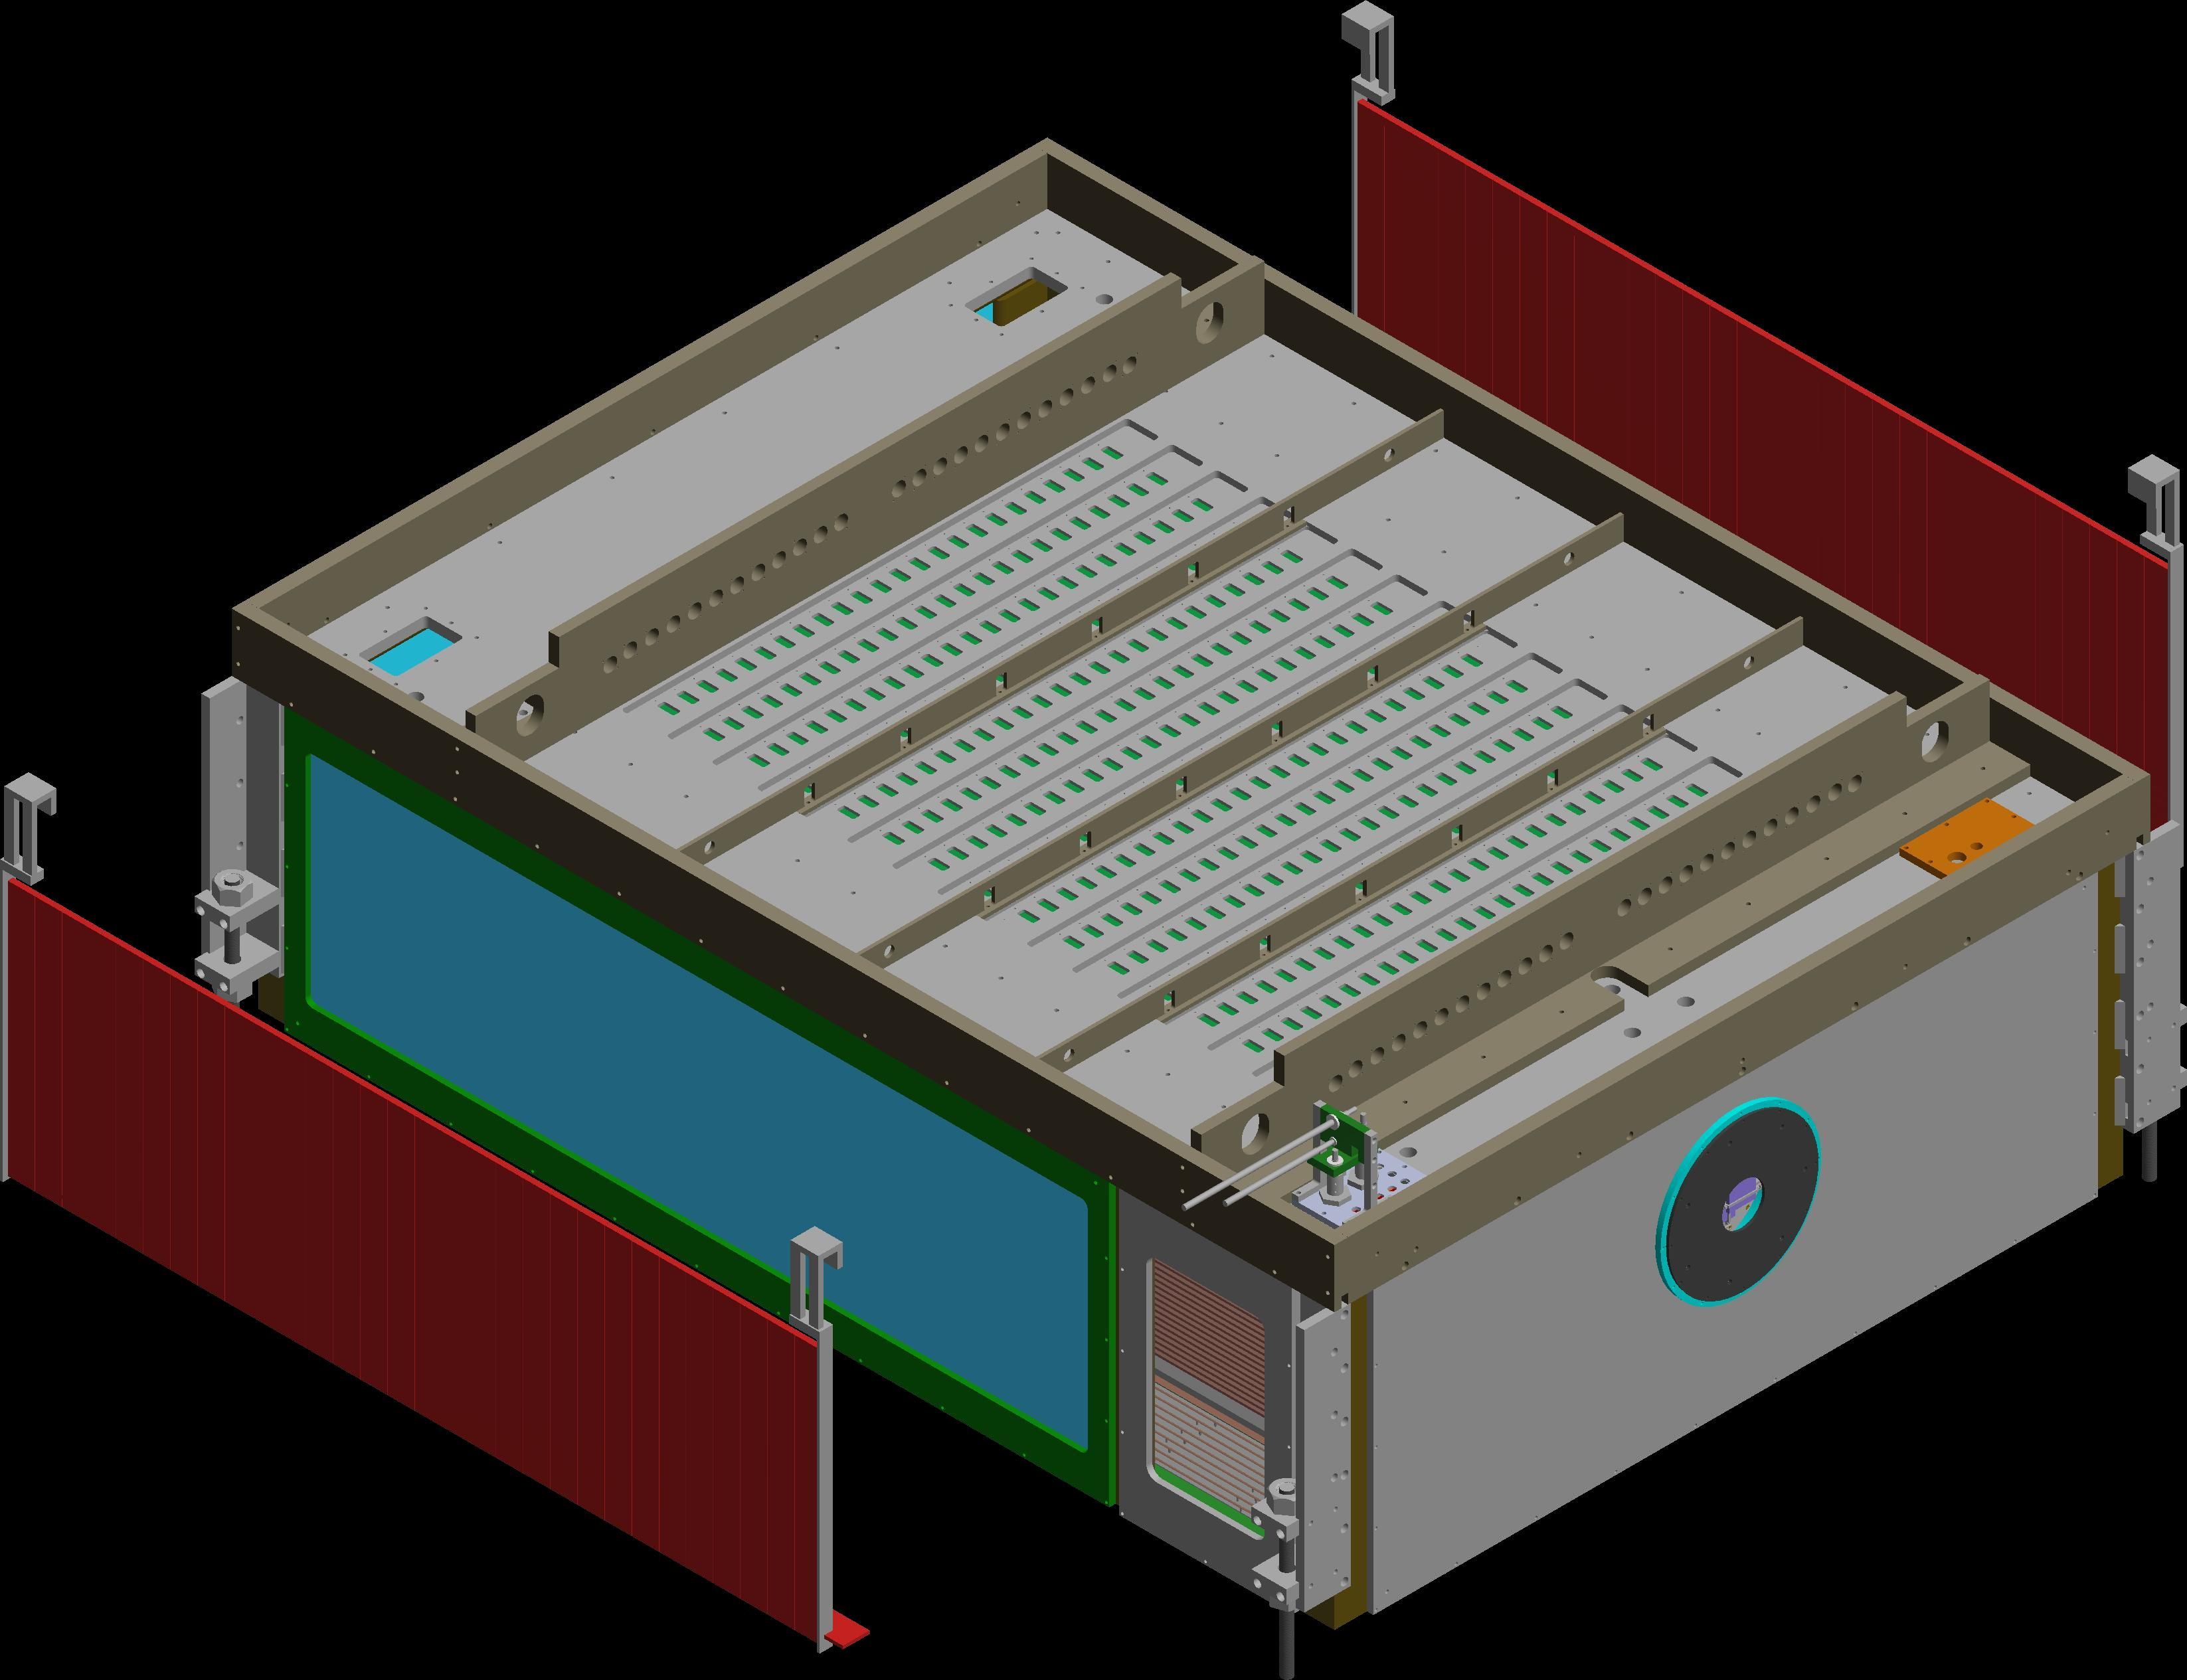
\includegraphics[width=\textwidth]{kyotoarray}
\label{fig:kyoto}
\caption{Kyoto array overview}
\end{figure}


\subsection{Krakow ?????? (KATANA)}
%beam veto
%beam trigger optional


\subsection{Active Veto Array}

\section{Radio Isotope Beam Factory (RIBF) Facility }
Cyclotron facility overview.
Samurai line overview.
Beam line element overview.
Big rips beam PID. reference 


\section{S$\pi$RIT at RIBF}
Picture of setup. 




SAMURAI (Superconducting Analyzer for Multi-particles from Radioisotope beams) is a large-acceptance multi-particle spectrometer for radioactive-beam experiments.
\begin{figure}[H]
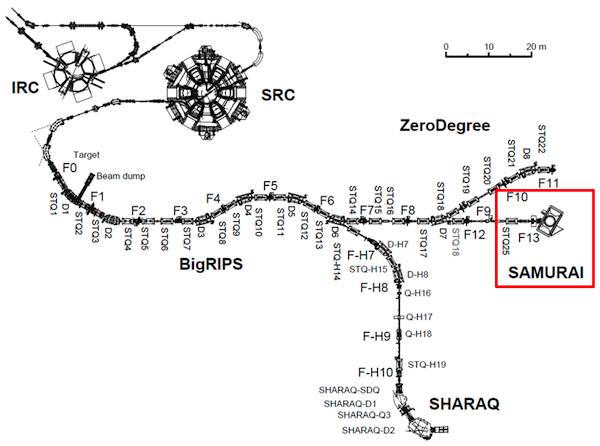
\includegraphics[width=\linewidth]{SAMURAI-beamline.png}
\caption{Overview of the RIBF, BigRIPS, and SAMURAI beamline.}
\label{fig:sambl}
\end{figure}

\section{Experimental Setup}

\section{Trigger Condition}
How it was made using kyoto krakow

\section{Collision Data Taken}

